\documentclass{beamer}
\setbeamertemplate{navigation symbols}{}

%\usepackage{beamerthemeshadow}
\usetheme{CambridgeUS}
\usecolortheme{beaver}
\setbeamerfont{frametitle}{size=\small}

\usepackage{xcolor}

\usepackage{nth}
\usepackage[export]{adjustbox}
\usepackage{tikz}
\usepackage{multirow}

\def\beamer@andinst{\quad}
\makeatother

\newcommand\parallelcontent[2]{
  \begin{columns}[t]
    \column{0.48\textwidth} #1
    \column{0.48\textwidth} #2
  \end{columns}
}
\newcommand\parallelitem[2]{
  \parallelcontent
  {\begin{itemize} \item #1 \end{itemize}}
  {\begin{itemize} \item[] #2 \end{itemize}}
}

\setbeamertemplate{caption}{\raggedright\insertcaption\par}

\usepackage{array}
\newcolumntype{L}[1]{>{\raggedright\let\newline\\\arraybackslash\hspace{0pt}}m{#1}}
\newcolumntype{C}[1]{>{\centering\let\newline\\\arraybackslash\hspace{0pt}}m{#1}}
\newcolumntype{R}[1]{>{\raggedleft\let\newline\\\arraybackslash\hspace{0pt}}m{#1}}

\newcommand{\specialcell}[2][c]{\begin{tabular}[#1]{@{}c@{}}#2\end{tabular}}

\newcommand{\includepatches}[1]{
	\includegraphics[width=0.13\textwidth]{pics/blobs/#1}
}

\newcommand{\nomargincell}[2][c]{
	\setlength\tabcolsep{0pt}
	\renewcommand{\arraystretch}{0.1}
	\begin{tabular}[#1]{@{}c@{}}#2\end{tabular}
	}


\begin{document}

\title{Diabetic Retinopathy Detection}
\subtitle{}  
\author[]{Sergey Ovcharenko \inst{1} \and Rasim Akhunzyanov \inst{2}}
\institute[shortinst]{\inst{1} Deep Learning Engineer at NTech Lab \and \inst{2} Computer Vision Research Engineer at LG Electronics}

\date{\today} 

\begin{frame}
\titlepage
\end{frame}

\begin{frame}
\frametitle{Table of contents}\tableofcontents
\end{frame} 

% % % %
% % % % Overview
% % % %
\section{Overview} 

\subsection{Competition Details}
\begin{frame}\frametitle{Data} 
\par \textbf{Goal}: Identify signs of diabetic retinopathy in eye images
\par \textbf{Given}: 35126 images for training, 53576 images in test set
\par Images are big: 2500x2000
\par Compressed data size: 88Gb

\vspace{5pt}

\begin{tabular}{|@{}c@{}|@{}c@{}|@{}c@{}|@{}c@{}|@{}c@{}|}
\hline
	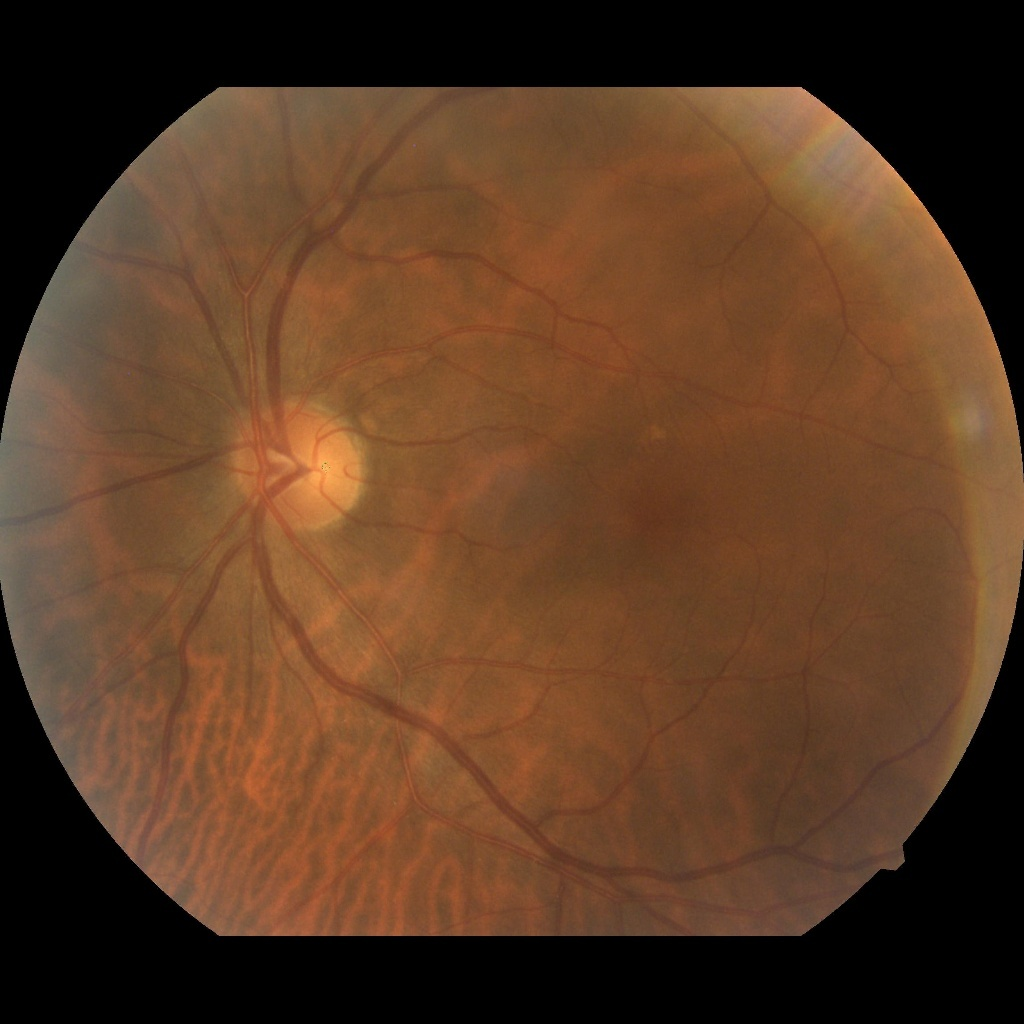
\includegraphics[width=0.2\textwidth]{pics/classified_samples/197_left_0.jpg} &
	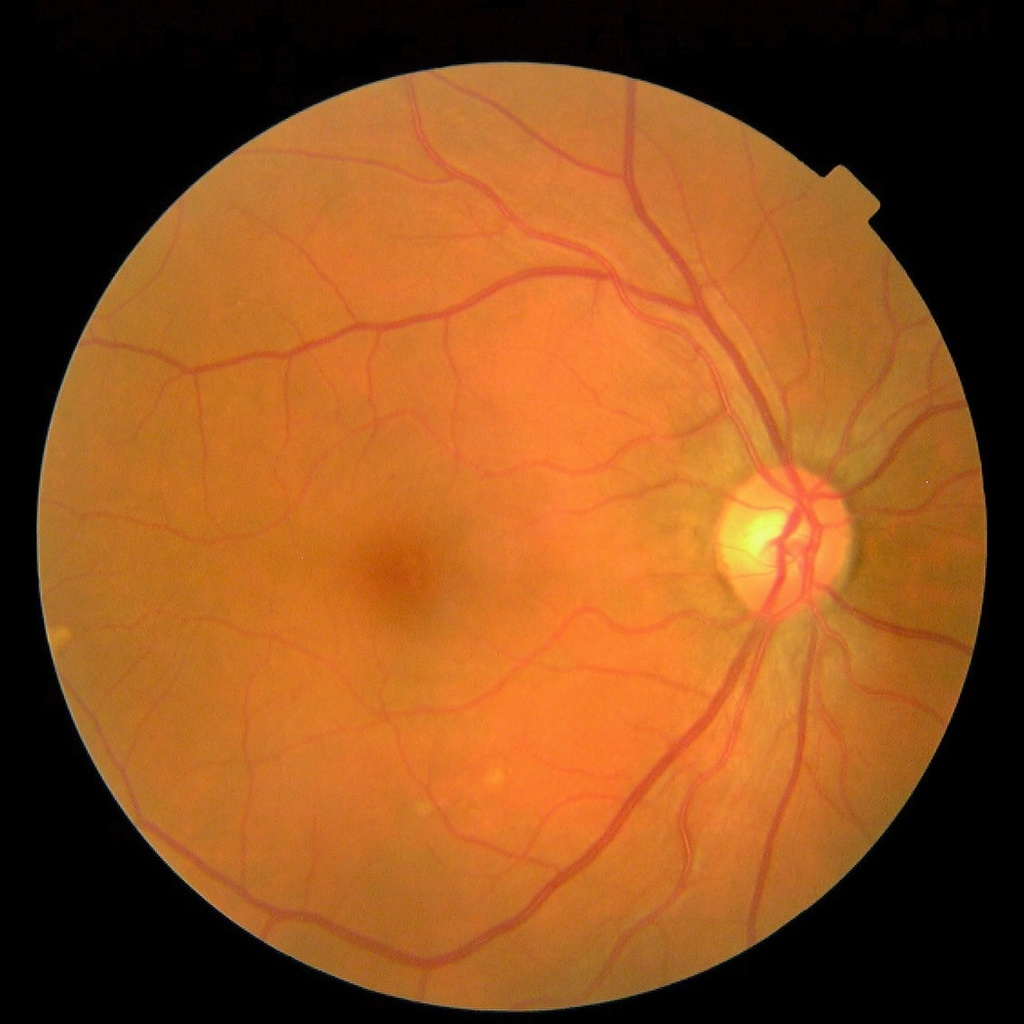
\includegraphics[width=0.2\textwidth]{pics/classified_samples/204_right_1.jpg} &
	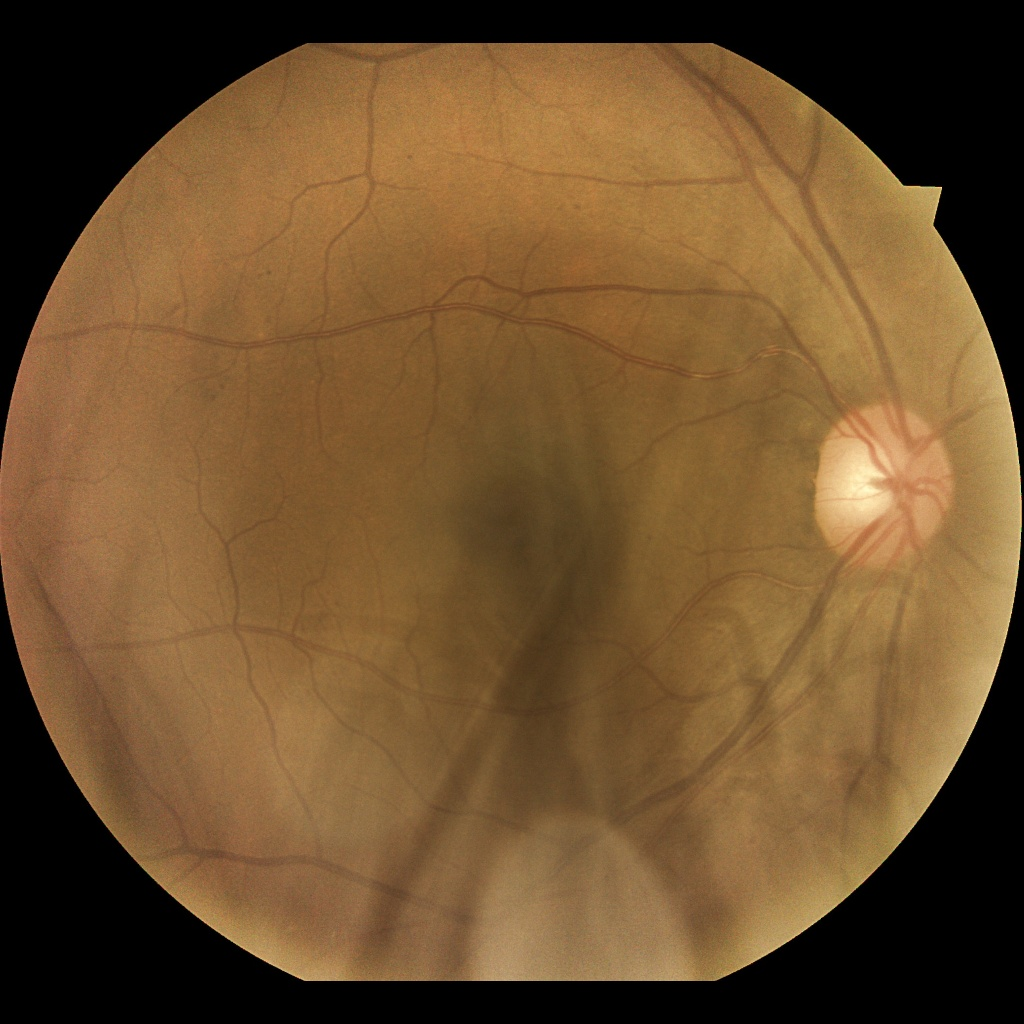
\includegraphics[width=0.2\textwidth]{pics/classified_samples/82_right_2.jpg} &
	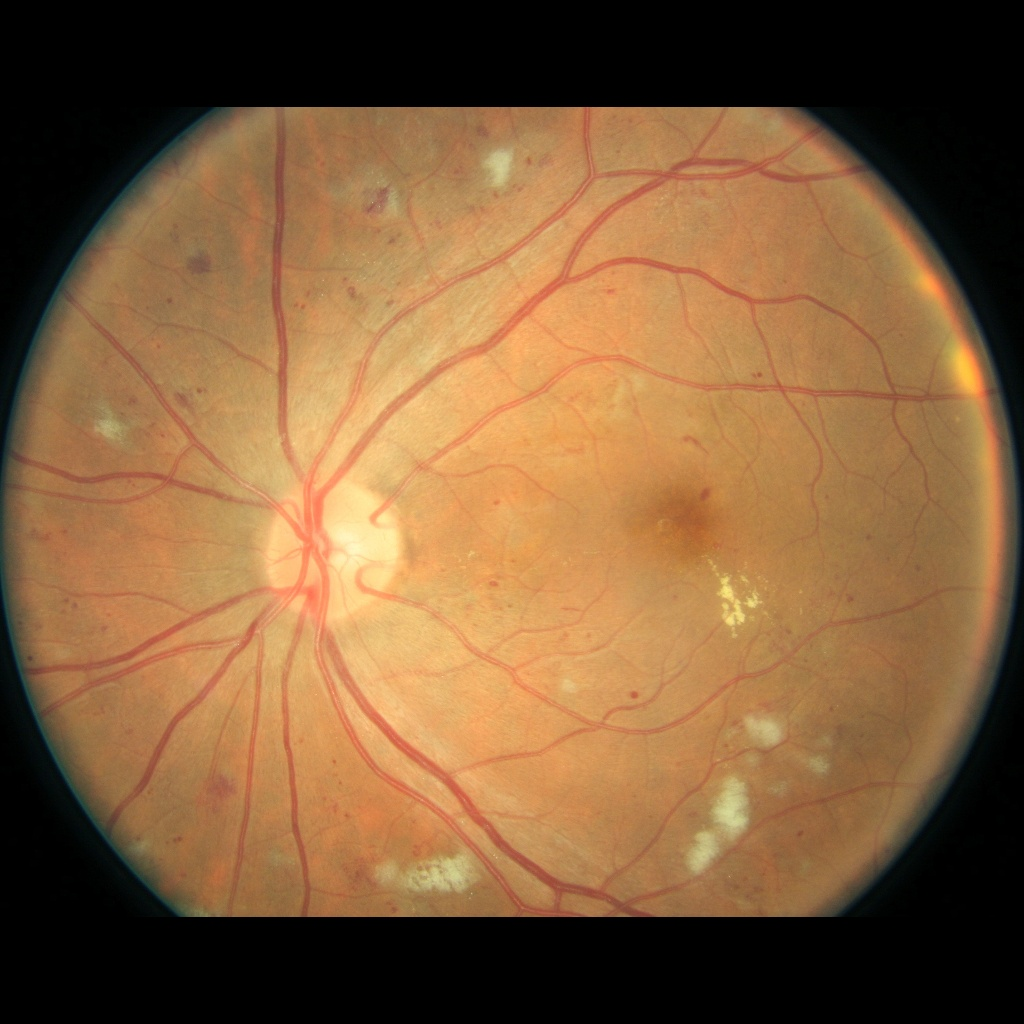
\includegraphics[width=0.2\textwidth]{pics/classified_samples/687_right_3.jpg} &
	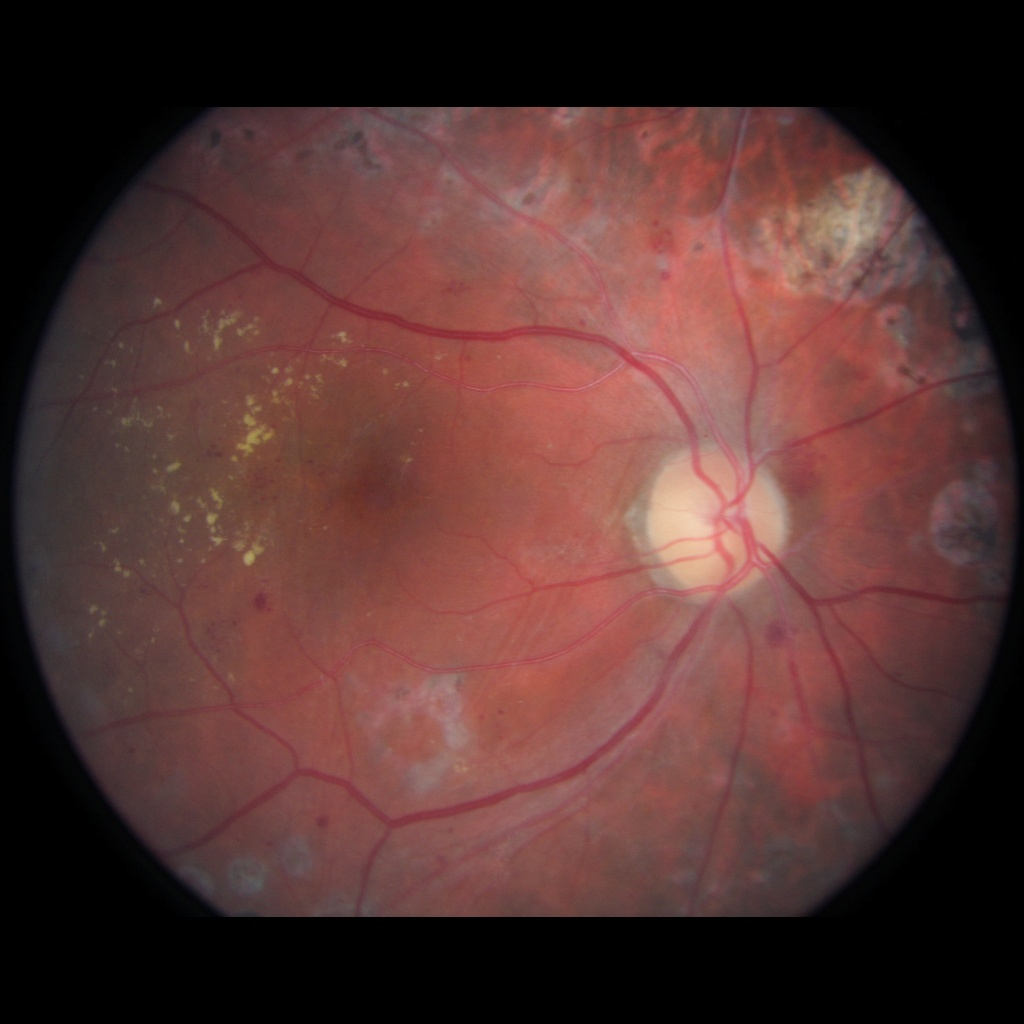
\includegraphics[width=0.2\textwidth]{pics/classified_samples/2496_left_4.jpg} \\\noalign{\vspace{-0.15cm}}
\hline

Normal & Mild & Moderate & Severe & Proliferative \\

\hline
 \specialcell{25810\\ \footnotesize{73.48\%}}  & 
 \specialcell{2443\\\footnotesize6.96\%} & 
 \specialcell{5292\\\footnotesize15.07\%} & 
 \specialcell{873\\\footnotesize2.48\%} & 
 \specialcell{708\\\footnotesize2.01\%} \\

\hline
\end{tabular}

\end{frame}

\begin{frame}\frametitle{Quality metric: quadratic weighted kappa} 

\footnotesize { % TODO: rewrite
Images have five possible ratings, 0,1,2,3,4.  Each image is characterized by a tuple $ (e_a,e_b) $, which corresponds to its scores by $Rater A$ (human) and $Rater B$ (predicted).  The quadratic weighted kappa is calculated as follows. First, an $N\times N$ histogram matrix $O$ is constructed, such that $O_{i,j}$ corresponds to the number of images that received a rating $i$ by $A$ and a rating $j$ by $B$. An $N\times N$ matrix of weights, $w$, is calculated based on the difference between raters' scores:

\[ w_{i,j} = \frac{\left(i-j\right)^2}{\left(N-1\right)^2} \]

An $N\times N$ histogram matrix of expected ratings, $E$, is calculated, assuming that there is no correlation between rating scores.  This is calculated as the outer product between each rater's histogram vector of ratings, normalized such that $E$ and $O$ have the same sum.

From these three matrices, the quadratic weighted kappa is calculated as: 

\[ \kappa=1-\frac{\sum_{i,j}w_{i,j}O_{i,j}}{\sum_{i,j}w_{i,j}E_{i,j}}. \]
}

\end{frame}

\subsection{Competition Results}

\begin{frame}\frametitle{} 
\begin{center}
\only<1>{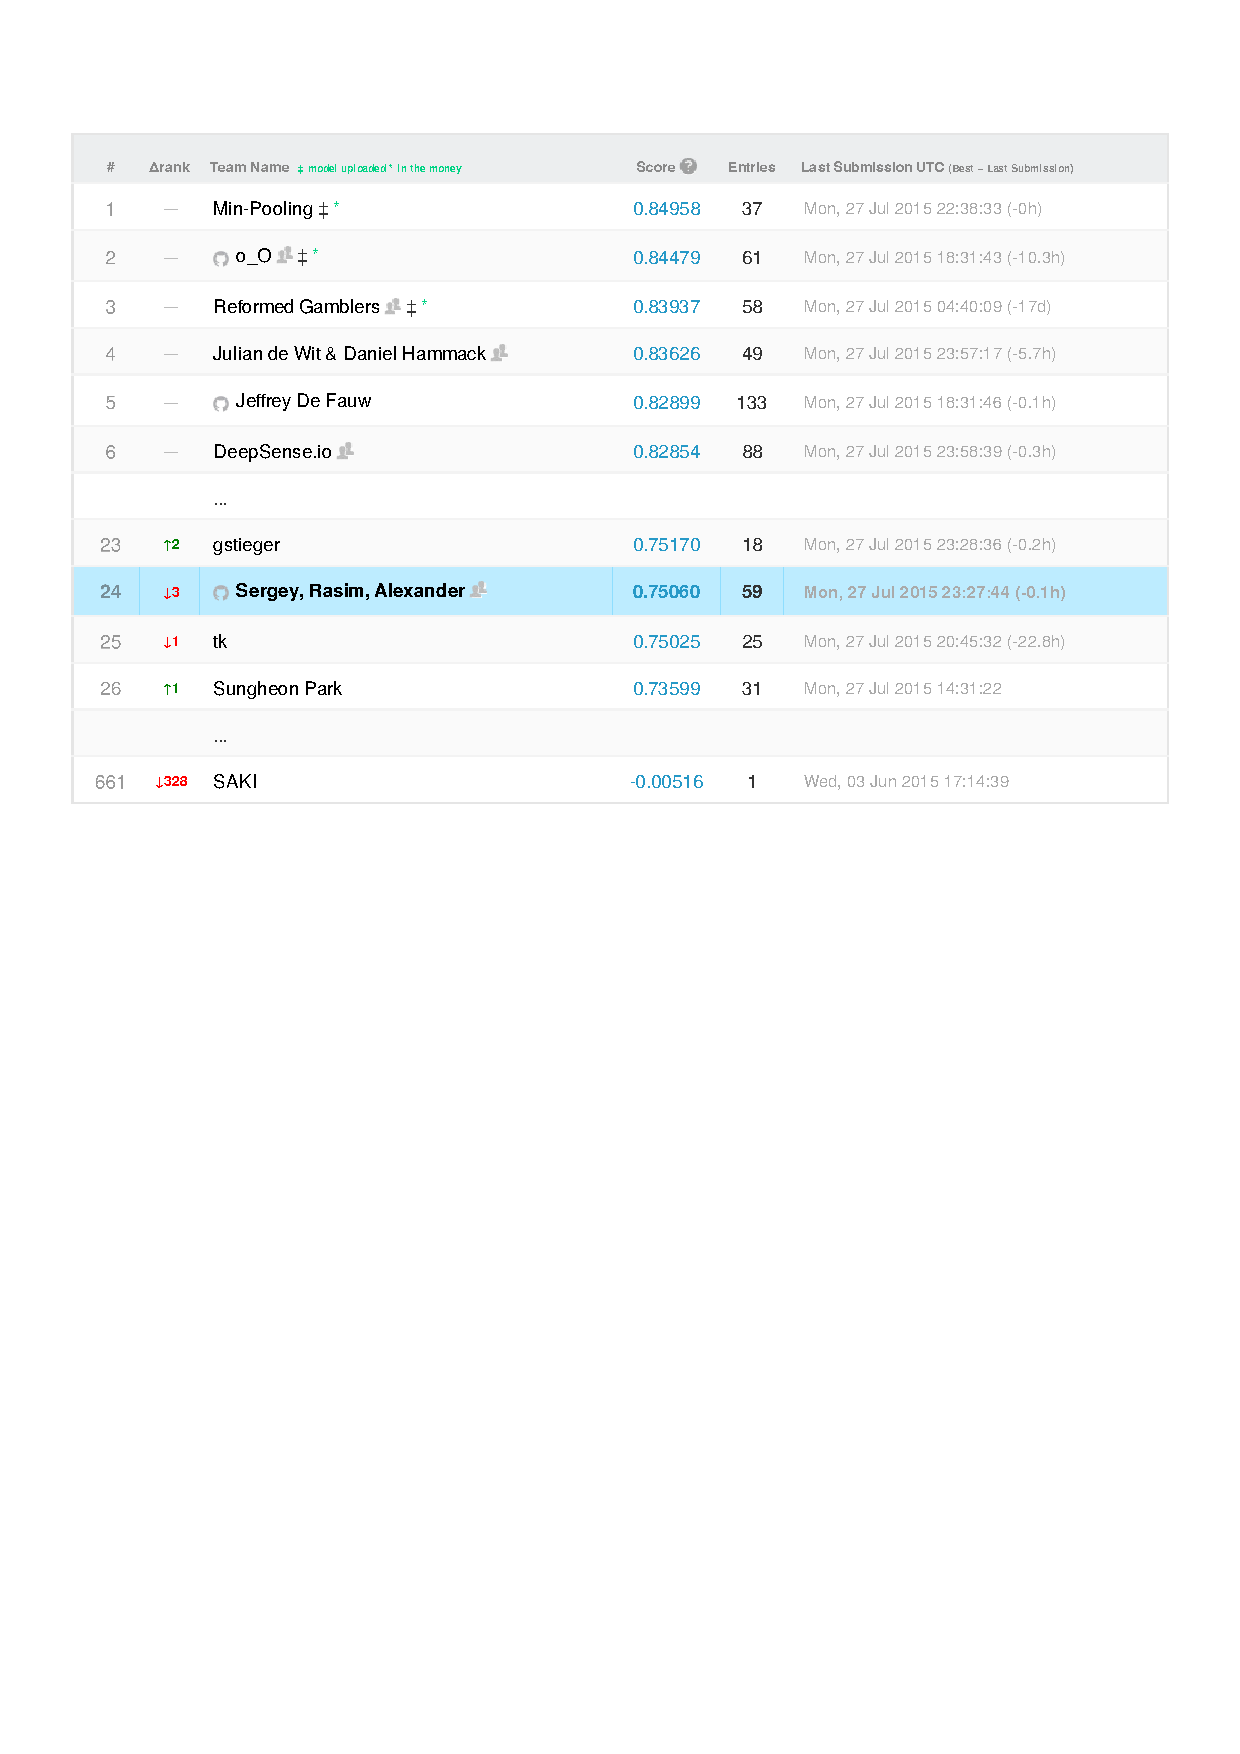
\includegraphics[width=\textwidth]{pics/private_lb_selected.pdf}}
\only<2>{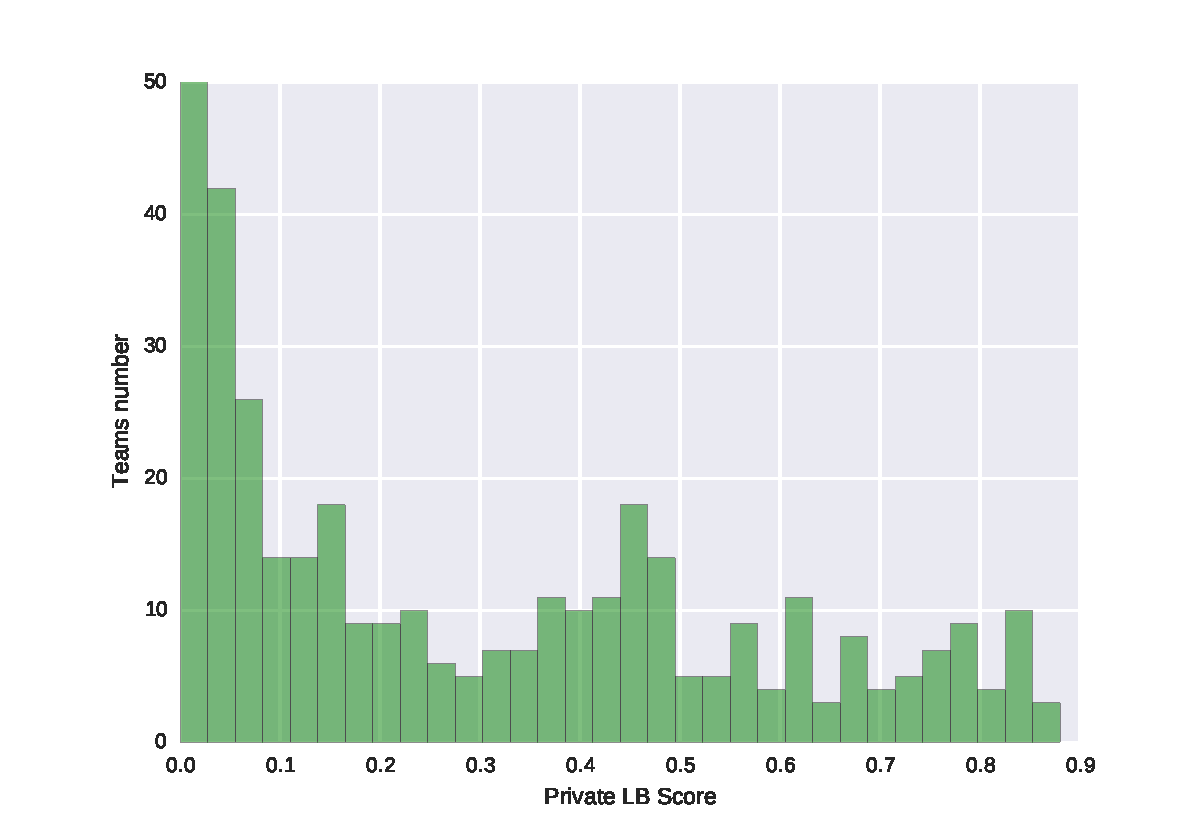
\includegraphics[width=\textwidth]{pics/private_lb_distribution.pdf}}
\only<3>{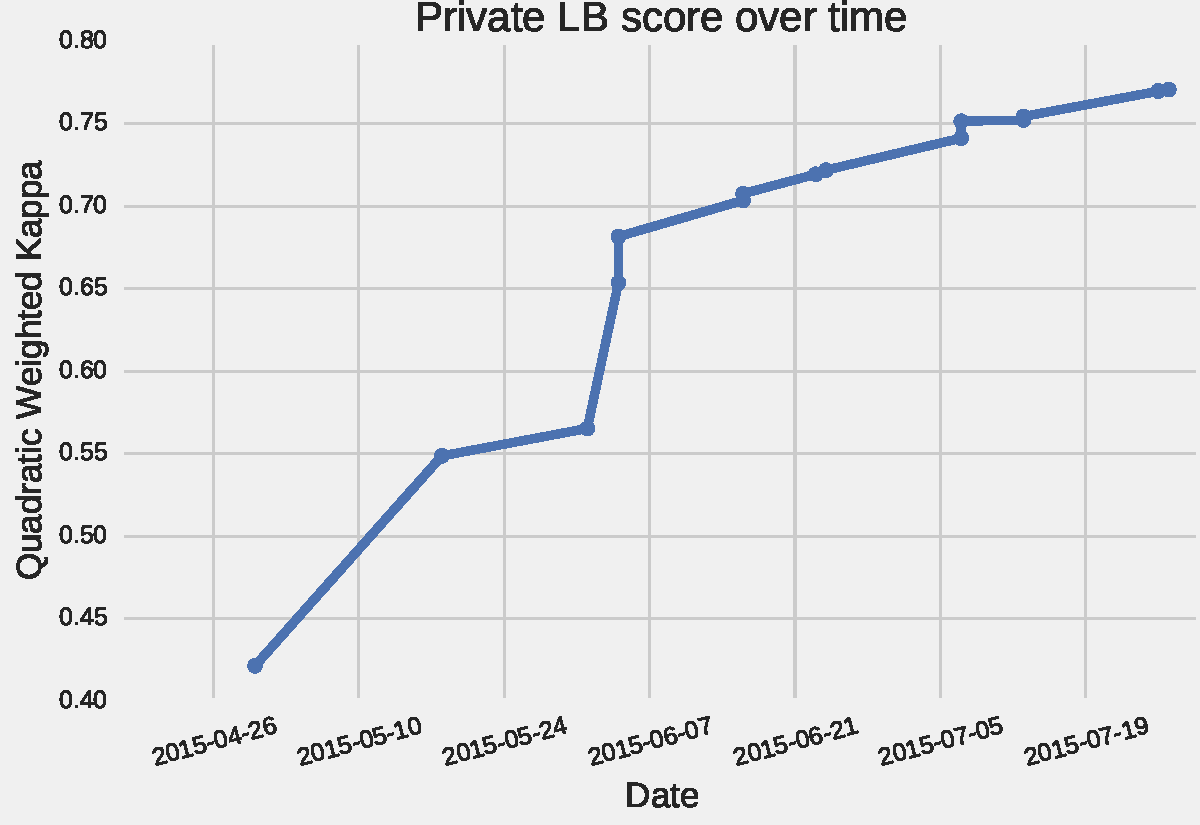
\includegraphics[width=\textwidth]{pics/private_lb_score_increase.pdf}}
\end{center}
\end{frame}

%\begin{frame}\frametitle{} 
%\par final leaderboard
%\par + provide leaderboard histogram
%\par + plot score over time
%\end{frame}

% % % %
% % % % Solution
% % % %
\section{Solution}

\begin{frame}\frametitle{Domain knowledge: diabetic retinopathy symptoms}

\begin{itemize}
\item {\hyperlink{https://goo.gl/s5lMt8}{DR symptoms cheatsheet: https://goo.gl/s5lMt8}
\begin{center}
\par 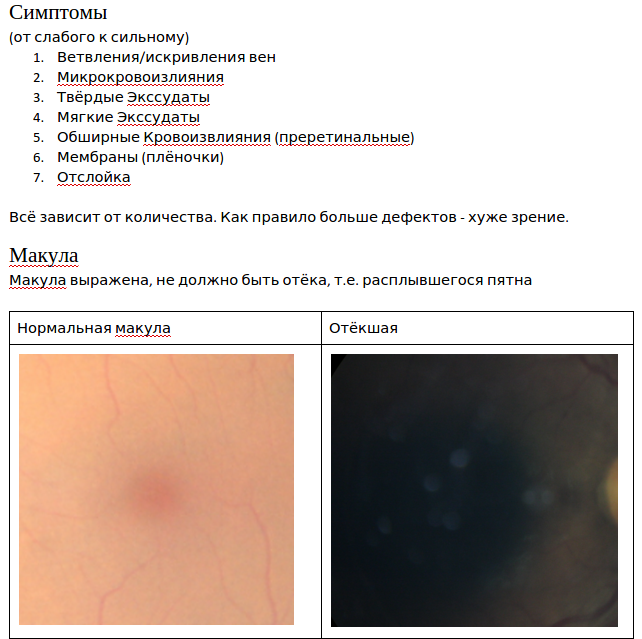
\includegraphics[interpolate=true,valign=c,width=0.4\textwidth]{pics/symptoms_pic.png}
\end{center}
Was prepared with assistance of Vera Shevchenko
}
\item \href{http://www.icoph.org/downloads/Diabetic-Retinopathy-Detail.pdf}{International Clinical Diabetic Retinopathy Disease Severity Scale, Detailed Table: \small http://www.icoph.org/downloads/Diabetic-Retinopathy-Detail.pdf}
\end{itemize}

\end{frame}

\subsection{Data preparation}


\begin{frame}\frametitle{Preprocessing}
\begin{columns}

\begin{column}{9cm}
\begin{itemize}
\item Crop black borders
\vspace{20pt}

\item Extent to square + resize
\vspace{20pt}

\item Optionally: crop internal square
\vspace{20pt}

\item Optionally: Local Contrast Normalization (LCN) \\ 
      $ \hat{I}_{x,y} = \frac{I_{x,y} - \mu_{x,y}}{\sigma_{x,y}} $
\end{itemize}
\end{column}

\begin{column}{6cm}
\begin{tabular}{ @{}c m{0.25cm} c }

	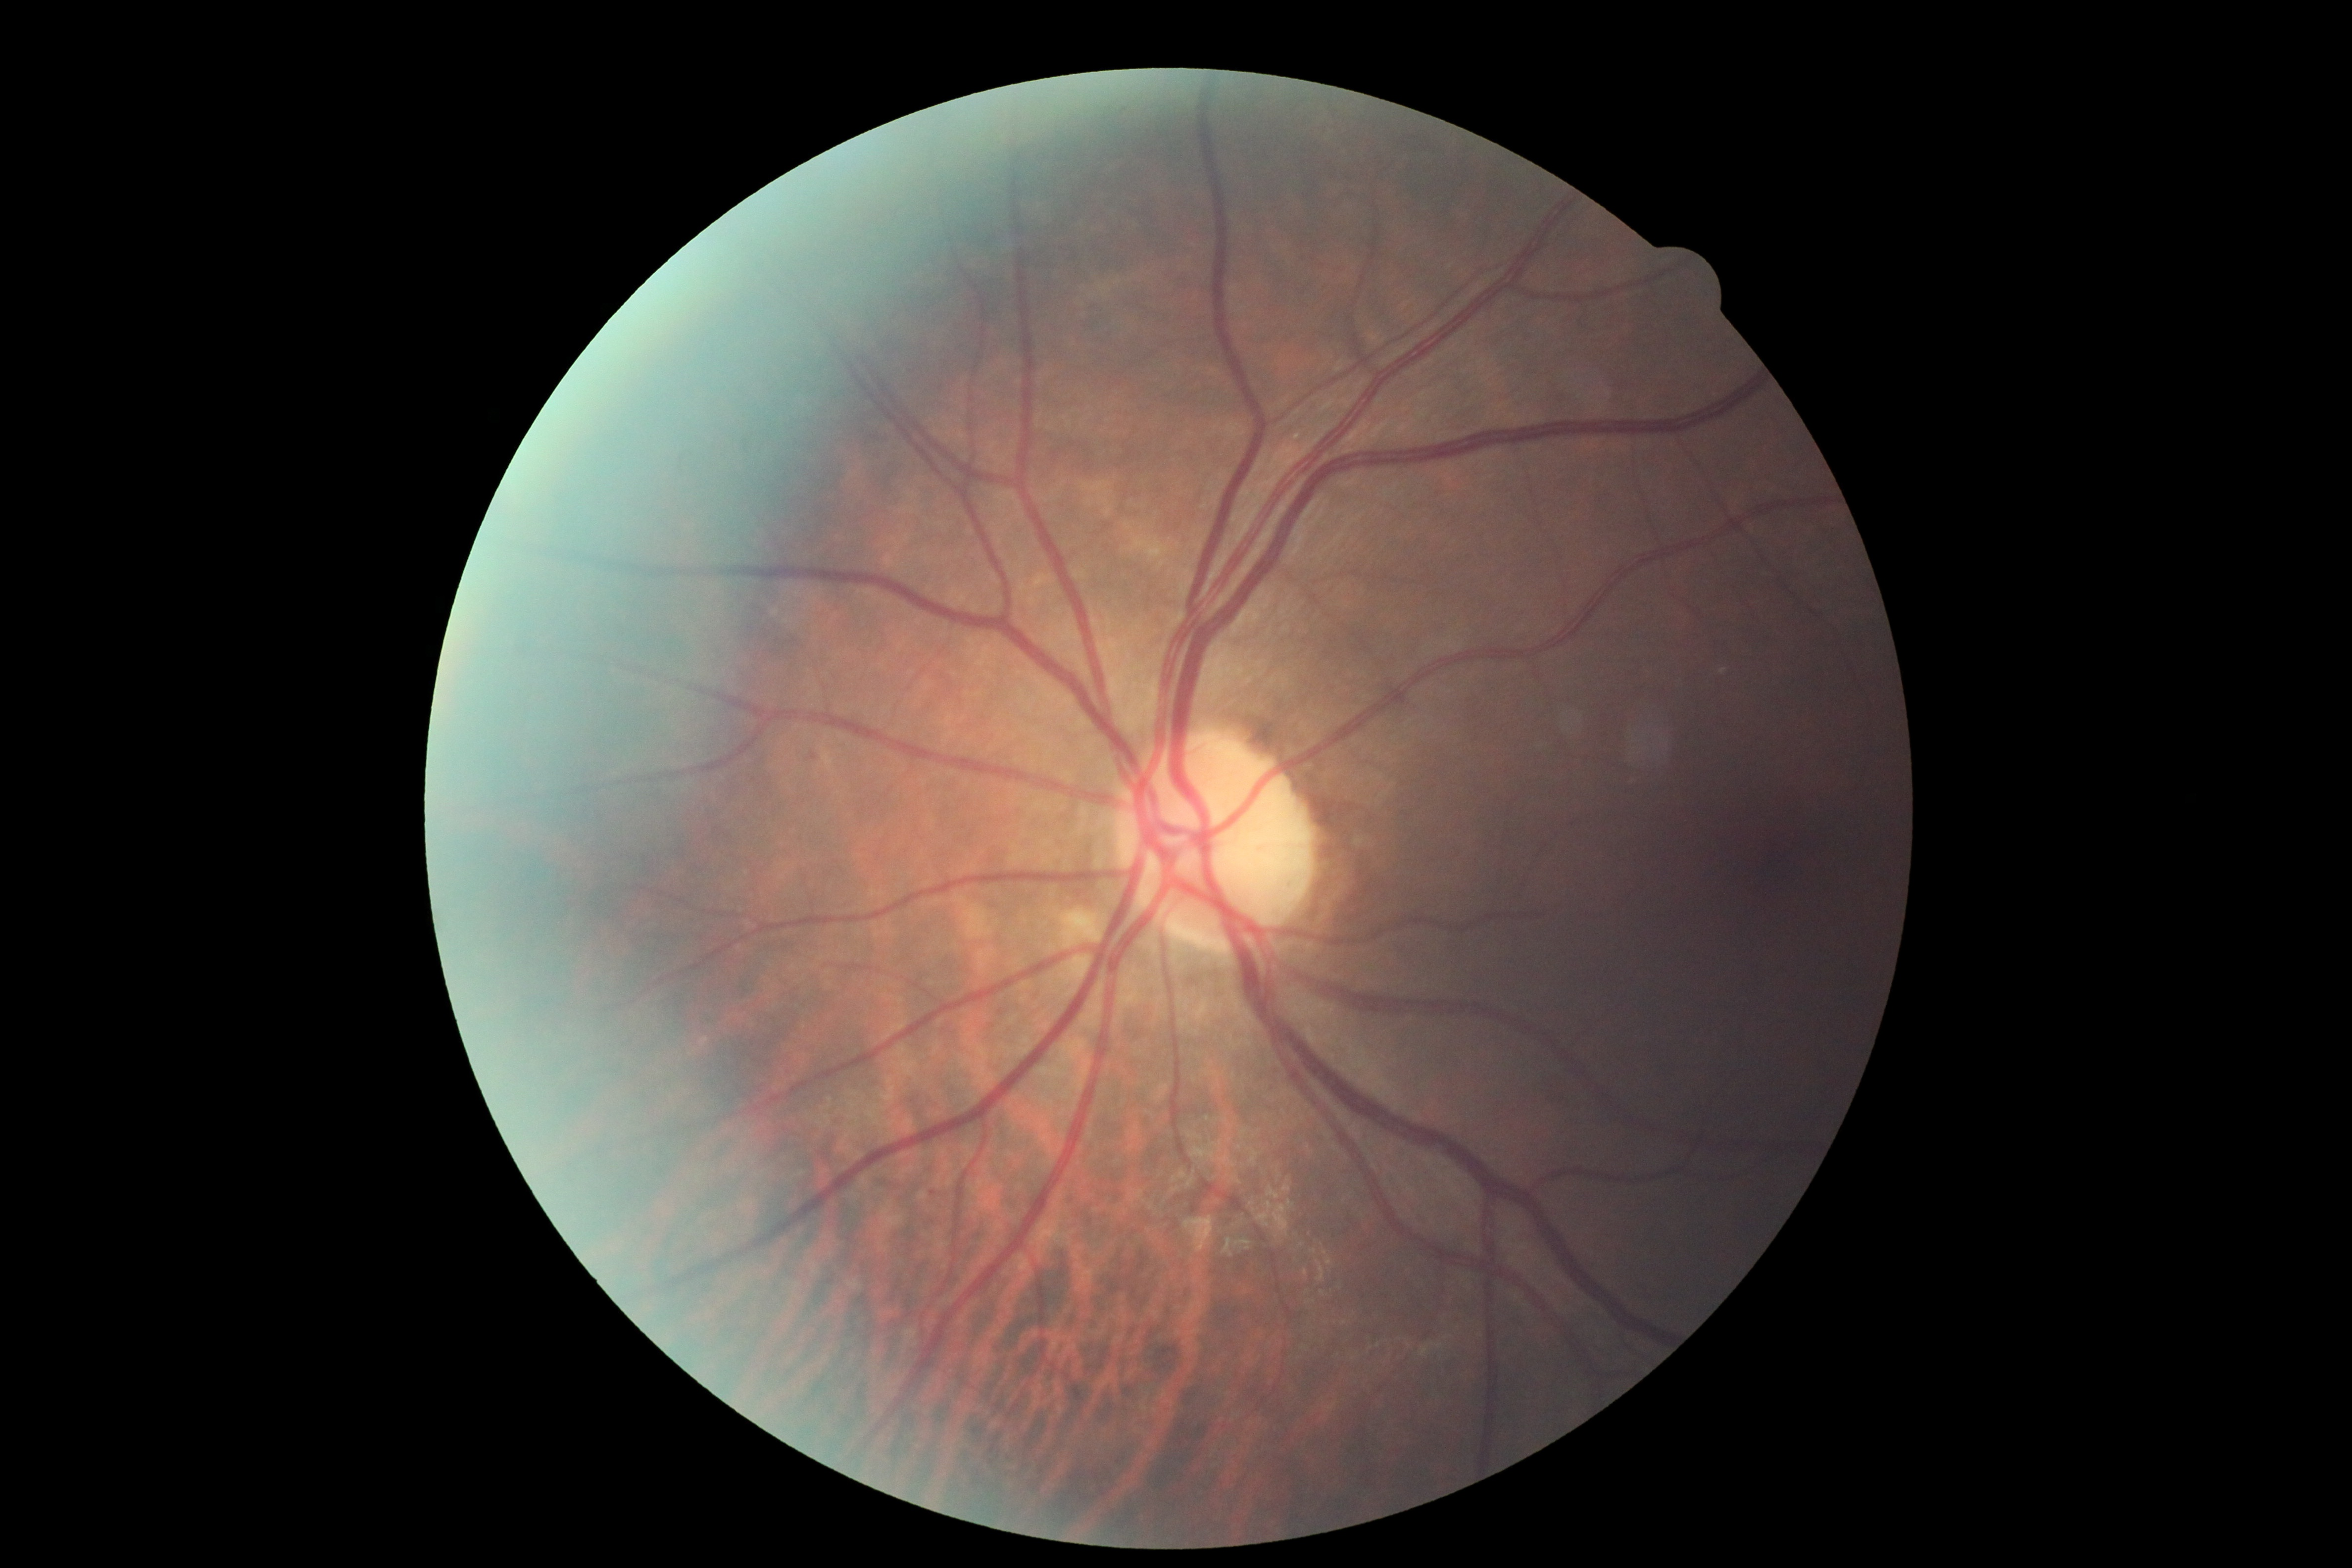
\includegraphics[valign=c,height=0.5cm]{pics/10_left.jpeg} & $\rightarrow$ &
    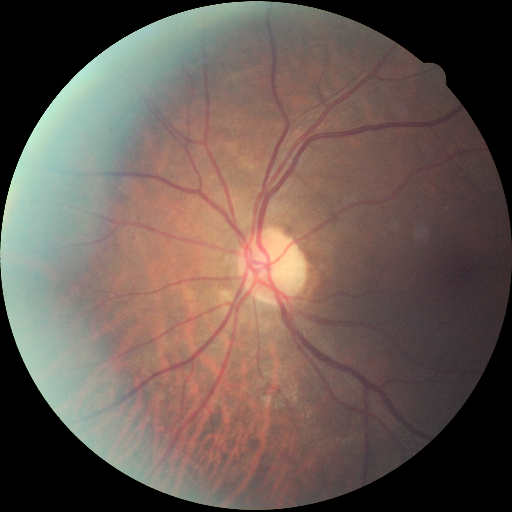
\includegraphics[valign=c,height=0.5cm]{pics/10_left.png}
    \vspace{10pt} \\ 
    
	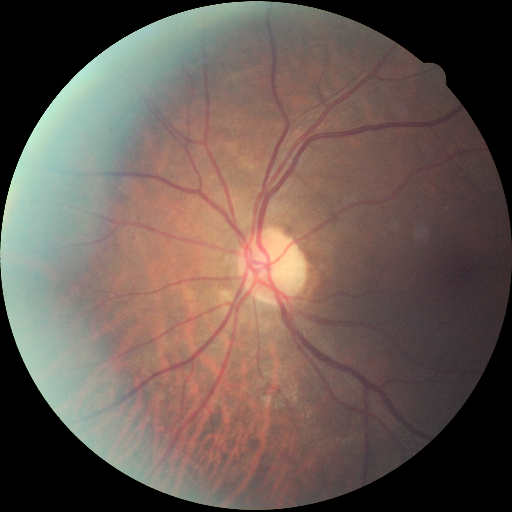
\includegraphics[valign=c,height=0.5cm]{pics/10_left.png} & $\rightarrow$ &
    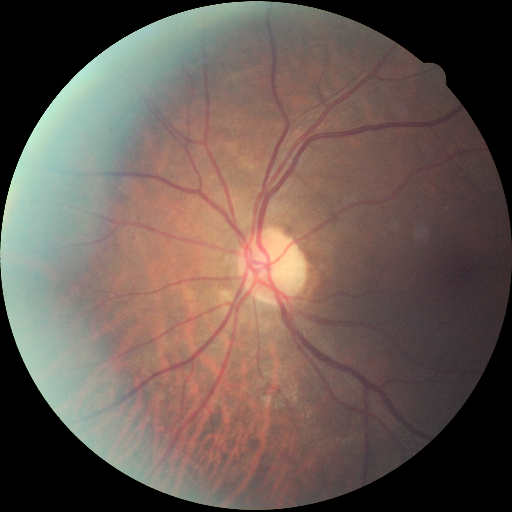
\includegraphics[valign=c,height=0.25cm]{pics/10_left.png}
	\vspace{10pt} \\ 	

	\adjustbox{valign=c}{\begin{tikzpicture}
	    \node[anchor=south west,inner sep=0] (image) at (0,0) {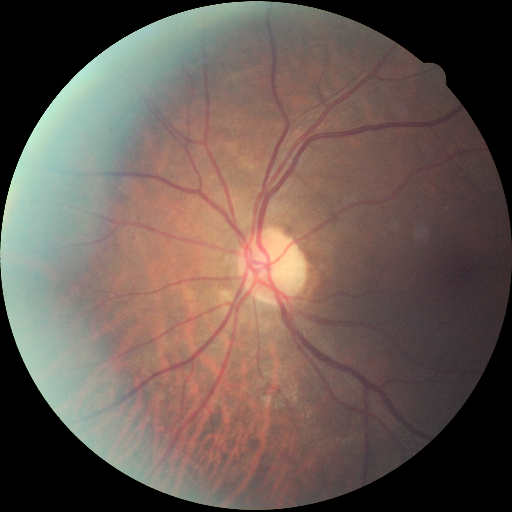
\includegraphics[valign=c,height=0.5cm]{pics/10_left.png}};
	        \begin{scope}[x={(image.south east)},y={(image.north west)}]
	            \draw[red] (0,0.5) -- (0.5,1) -- (1,0.5) -- (0.5,0) -- (0,0.5);
	        \end{scope}
	\end{tikzpicture}} & $\rightarrow$ &
	    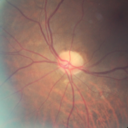
\includegraphics[valign=c,height=0.5cm]{pics/10_left_inner.png}
    \vspace{10pt} \\

%    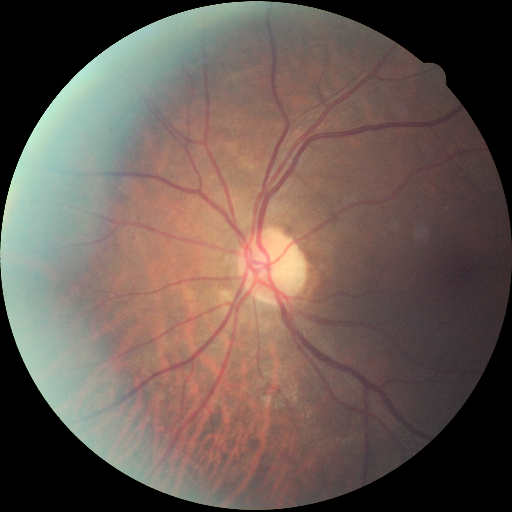
\includegraphics[valign=c,height=0.5cm]{pics/10_left.png} & $\rightarrow$ &
%    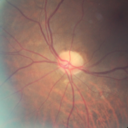
\includegraphics[valign=c,height=0.5cm]{pics/10_left_inner.png}
%	\vspace{10pt} \\

	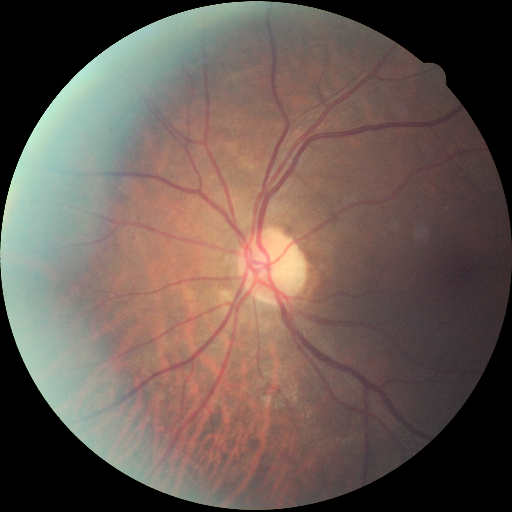
\includegraphics[valign=c,height=0.5cm]{pics/10_left.png} & $\rightarrow$ &
	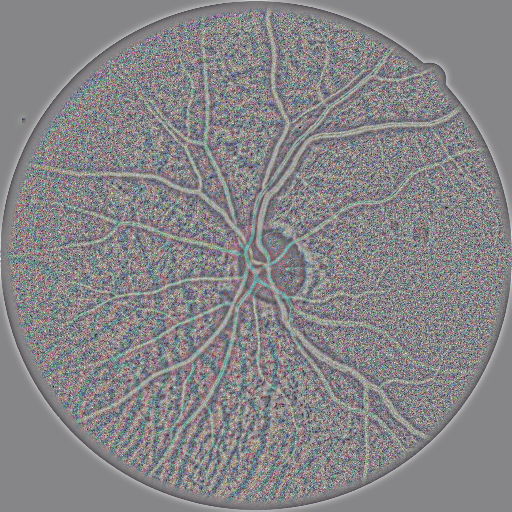
\includegraphics[valign=c,height=0.5cm]{pics/10_left_lcn.png}
	\\


\end{tabular}
\end{column}

\end{columns}
\end{frame}

\begin{frame}\frametitle{Augmentation}
\begin{itemize}
\item Random mirror
\item Random rotation
\item Color augmentation - not helped
\end{itemize}

\end{frame}

\subsection{Network configuration}
\begin{frame}\frametitle{}
\par Slice rotate
\par Merge
\par Output
\end{frame}

\subsection{Network configuration}
\begin{frame}\frametitle{}

\begin{table}[]
\tiny	
\centering
\begin{tabular}{@{}lll@{}}
Layer type & Size & Output shape \\
cyclic slice &  & (128, 1, 95, 95) \\
convolution & 32 3x3 filters & (128, 32, 95, 95) \\
convolution & 16 3x3 filters & (128, 16, 95, 95) \\
max pooling & 3x3, stride 2 & (128, 16, 47, 47) \\
cyclic roll &  & (128, 64, 47, 47) \\
convolution & 64 3x3 filters & (128, 64, 47, 47) \\
convolution & 32 3x3 filters & (128, 32, 47, 47) \\
max pooling & 3x3, stride 2 & (128, 32, 23, 23) \\
cyclic roll &  & (128, 128, 23, 23) \\
convolution & 128 3x3 filters & (128, 128, 23, 23) \\
convolution & 128 3x3 filters & (128, 128, 23, 23) \\
convolution & 64 3x3 filters & (128, 64, 23, 23) \\
max pooling & 3x3, stride 2 & (128, 64, 11, 11) \\
cyclic roll &  & (128, 256, 11, 11) \\
convolution & 256 3x3 filters & (128, 256, 11, 11) \\
convolution & 256 3x3 filters & (128, 256, 11, 11) \\
convolution & 128 3x3 filters & (128, 128, 11, 11) \\
max pooling & 3x3, stride 2 & (128, 128, 5, 5) \\
cyclic roll &  & (128, 512, 5, 5) \\
fully connected & 512 2-piece maxout units & (128, 512) \\
cyclic pooling (rms) &  & (32, 512) \\
fully connected & 512 2-piece maxout units & (32, 512) \\
fully connected & 121-way softmax & (32, 121)
\end{tabular}
\end{table}
\end{frame}


\subsection{Decision making}

\begin{frame}\frametitle{}
\par Predict score for eyes independently
\par Final score = max(left, right)
\end{frame}


\section{Microaneurysm detection}

\subsection{Motivation}
\begin{frame}\frametitle{Motivation I}

\par Microaneurysms are early symptoms of diabetic retinopathy
\vspace{-20pt}

\begin{table}[]
\begin{tabular}{|p{2cm}|p{8cm}|}
\hline
Disease level &  Findings observable upon dilated ophthalmoscopy \\ \hline
\footnotesize None &  No abnormalities \\ \hline
\footnotesize Mild NPDR & { Microaneurysms only} \\ \hline
\footnotesize Moderate NDPR &  More than just MA but less than severe NPDR \\ \hline
\multirow{4}{*}{\footnotesize Severe NPDR} & \multirow{4}{*}{\begin{tabular}[c]{@{}l@{}}
 $>$20 intraretinal hemorrhages in each quad \\
or  Definite venous beading in 2+ quads \\
or  Intraretinal microvascular anomalies in 1+ quad \end{tabular}} \\
 &  \\
 &  \\
 &  \\ \hline
\footnotesize PDR & \begin{tabular}[c]{@{}l@{}} Neovascularization\\  or/and Vitreous/preretinal hemorrhage\end{tabular} \\ \hline
\end{tabular}
\end{table}

\par \href{http://www.icoph.org/downloads/Diabetic-Retinopathy-Detail.pdf}{\footnotesize International Clinical Diabetic Retinopathy Disease Severity Scale, Detailed Table:  http://www.icoph.org/downloads/Diabetic-Retinopathy-Detail.pdf}

\end{frame}

\begin{frame}\frametitle{Motivation II}
\par We have problems with detection of early symptoms
\par
\begin{figure}
\begin{center}
\vspace{-10pt}
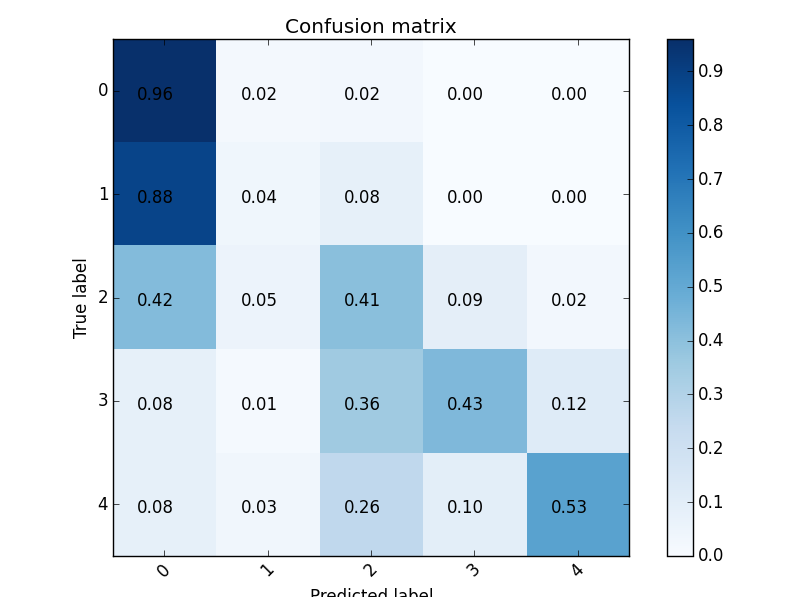
\includegraphics[width=0.4\textwidth]{pics/submission_21_inner_squares_conv5_maxout.png}
\caption{Confusion matrix on 128x128 pixels input}
\vspace{-15pt}
\end{center}
\end{figure}

\par MA have round shape with 2-5 pixels in radius on 1024x1024 image 
\par MA became invisible after downsampling to 128x128/256x256
\par $\Rightarrow$ Classes 0,1,2 almost indistinguishable due to low resolution
\par We have not enough resources\&data to learn on highres images
\par $\Rightarrow$ Let's try plain old image processing

\end{frame}

\subsection{Hessian blob detector} 
\small

\begin{frame}\frametitle{Microaneurysm candidates using the determinant of the Hessian I}

We want to know how much pixel location is similar to blob shape. Let's calculate Hessian matrix at that point:

\[
H(\mathbf{x}) = 
\begin{bmatrix}
L_{xx}(\mathbf{x}) & L_{xy}(\mathbf{x})\\
L_{xy}(\mathbf{x}) & L_{yy}(\mathbf{x})\\
\end{bmatrix}
\]

\begin{itemize}
\item $L_{aa}(\mathbf{x})$ is second partial derivative in the $a$ direction 
\item $L_{ab}(\mathbf{x})$ is the mixed partial second derivative in the $a$ and $b$ directions.
\end{itemize}

\par Derivatives are computed in some scale $\sigma_I$ -- smoothed by a Gaussian kernel
 \[L(\mathbf{x}) = g(\sigma_I) \otimes I(\mathbf{x}) .\]

\par Derivatives must be scaled by factor related to the Gaussian kernel: $\sigma_I^2$.

\end{frame}

\begin{frame}\frametitle{Microaneurysm candidates using the determinant of the Hessian II}

\par At each scale, \textbf{blobs points} are those points that are local extrema of determinant the Hessian matrix. 

\[ \operatorname{det} H(x; \sigma) = \sigma_I^2 ( L_{xx}L_{yy}(\mathbf{x}) - L_{xy}^2(\mathbf{x})) \]

\par Sign of the trace of Hessian matrix help distinguish dark from light points:
\[ \operatorname{trace} H(x; \sigma) = \sigma_I (L_{xx} + L_{yy}). \]

\par Straightforward differential blob detector with automatic scale selection:

\[ 
	(\hat{x}, \hat{\sigma}) = 
	\operatorname{argmaxlocal}_{(x; t)} ( \operatorname{det} H(x; \sigma) ) 
\]

\end{frame}

\newcommand{\includehessiangraphics}[1]{
	\adjincludegraphics[width=0.125\textwidth,trim={{.4\width} {.4\width} {.4\width} {.4\width}},clip]{#1}
}


\begin{frame}\frametitle{Microaneurysm candidates}

\begin{columns}
\begin{column}{1cm}

	\centering

	\par 687\_right

	\adjincludegraphics[width=1.5cm,trim={{.4\width} {.4\width} {.4\width} {.4\width}},clip]{pics/classified_samples/687_right_3.jpg}

	\adjincludegraphics[width=1.5cm,trim={{.4\width} {.4\width} {.4\width} {.4\width}},clip]{pics/classified_samples/687_right_3_high_contrast.jpg}

\end{column}
\begin{column}{11cm}


\begin{tabular}[ht]{ >{\centering\bfseries}m{2cm} @{}c@{}@{}c@{}@{}c@{}@{}c@{}@{}c@{}}
\toprule
 & $\sigma = 1.7$ & $\sigma = 3.4$ & $\sigma =  5.1$ & $\sigma = 6.8$ & $\sigma = 8.0$ \\
\midrule
$L_{xx}$ & 
	\includehessiangraphics{{pics/det_hessian/Lxx_3_000000}.png} &
	\includehessiangraphics{{pics/det_hessian/Lxx_7_000000}.png} &	\includehessiangraphics{{pics/det_hessian/Lxx_15_000000}.png} &	\includehessiangraphics{{pics/det_hessian/Lxx_21_000000}.png} &	\includehessiangraphics{{pics/det_hessian/Lxx_31_000000}.png} \\

$L_{xy}$ &
	\includehessiangraphics{{pics/det_hessian/Lxy_3_000000}.png} &
	\includehessiangraphics{{pics/det_hessian/Lxy_7_000000}.png} &	\includehessiangraphics{{pics/det_hessian/Lxy_15_000000}.png} &	\includehessiangraphics{{pics/det_hessian/Lxy_21_000000}.png} &	\includehessiangraphics{{pics/det_hessian/Lxy_31_000000}.png} \\
	
$L_{yy}$ &
	\includehessiangraphics{{pics/det_hessian/Lyy_3_000000}.png} &
	\includehessiangraphics{{pics/det_hessian/Lyy_7_000000}.png} &	\includehessiangraphics{{pics/det_hessian/Lyy_15_000000}.png} &	\includehessiangraphics{{pics/det_hessian/Lyy_21_000000}.png} &	\includehessiangraphics{{pics/det_hessian/Lyy_31_000000}.png} \\

$\operatorname{det} H(x; \sigma)$ & 
	\includehessiangraphics{{pics/det_hessian/DH_3_000000}.png} &
	\includehessiangraphics{{pics/det_hessian/DH_7_000000}.png} &	\includehessiangraphics{{pics/det_hessian/DH_15_000000}.png} &	\includehessiangraphics{{pics/det_hessian/DH_21_000000}.png} &	\includehessiangraphics{{pics/det_hessian/DH_31_000000}.png} \\
\bottomrule
\end{tabular}

\end{column}
\end{columns}


\end{frame}

\begin{frame}\frametitle{Microaneurysm candidates}
\centering
\only<1>{
\begin{tabular}{|@{}c@{}|@{}c@{}|@{}c@{}|@{}c@{}|@{}c@{}|}
\hline

Normal & Mild & Moderate & Severe & Proliferative \\

\hline
	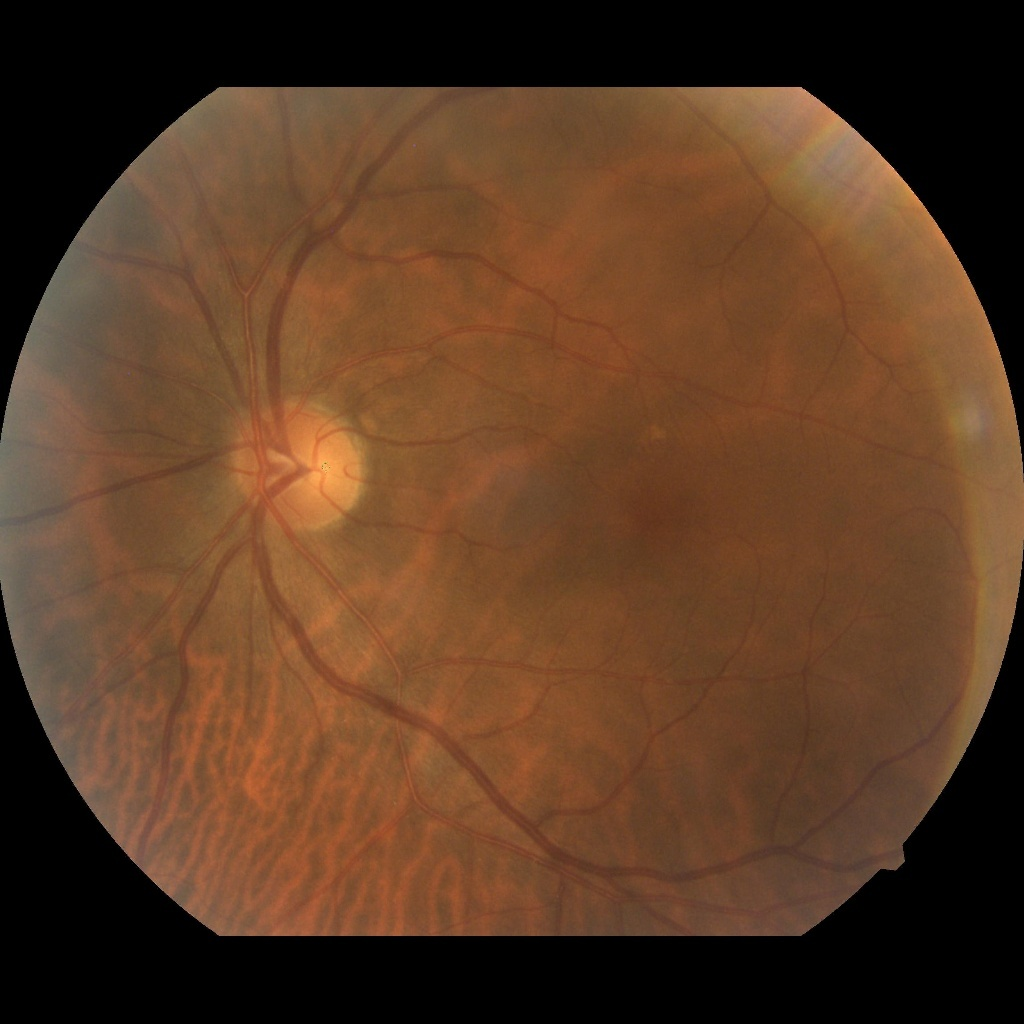
\includegraphics[width=0.2\textwidth]{pics/classified_samples/197_left_0.jpg} &
	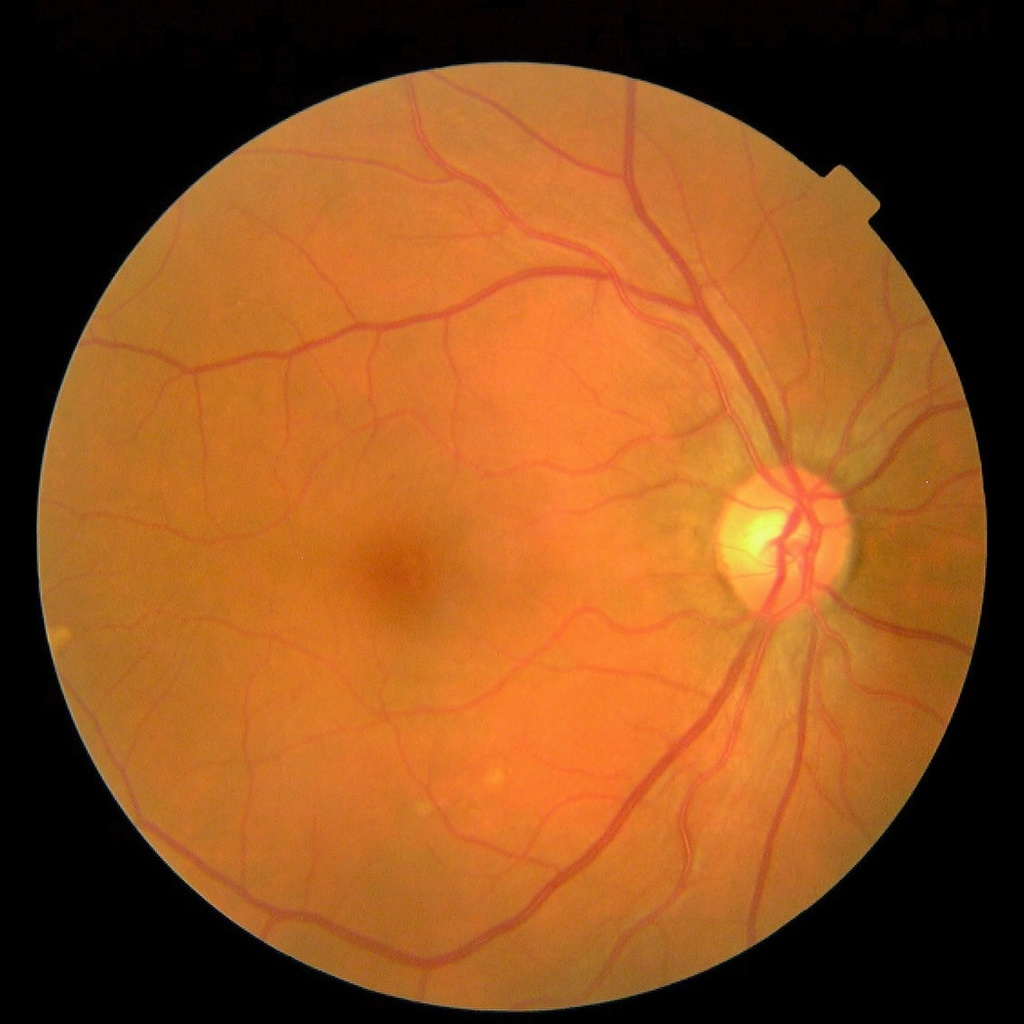
\includegraphics[width=0.2\textwidth]{pics/classified_samples/204_right_1.jpg} &
	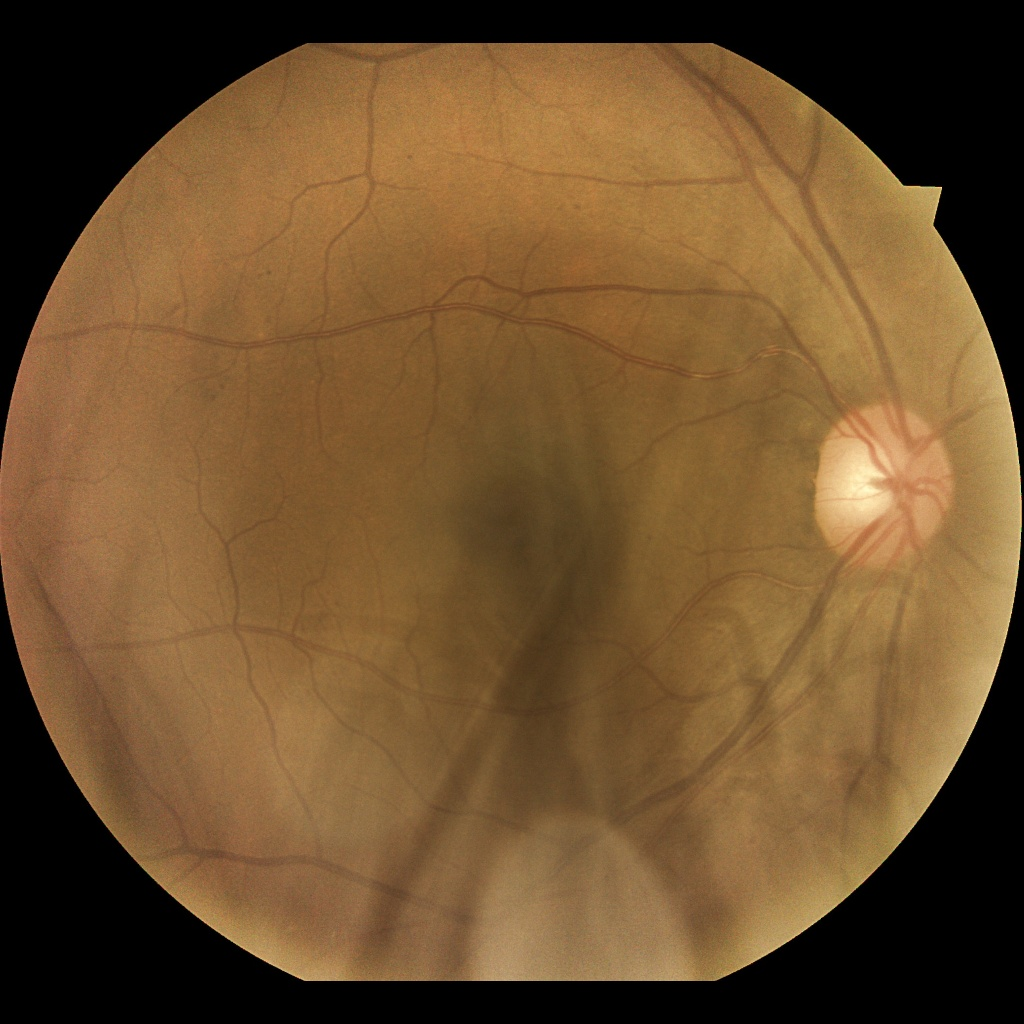
\includegraphics[width=0.2\textwidth]{pics/classified_samples/82_right_2.jpg} &
	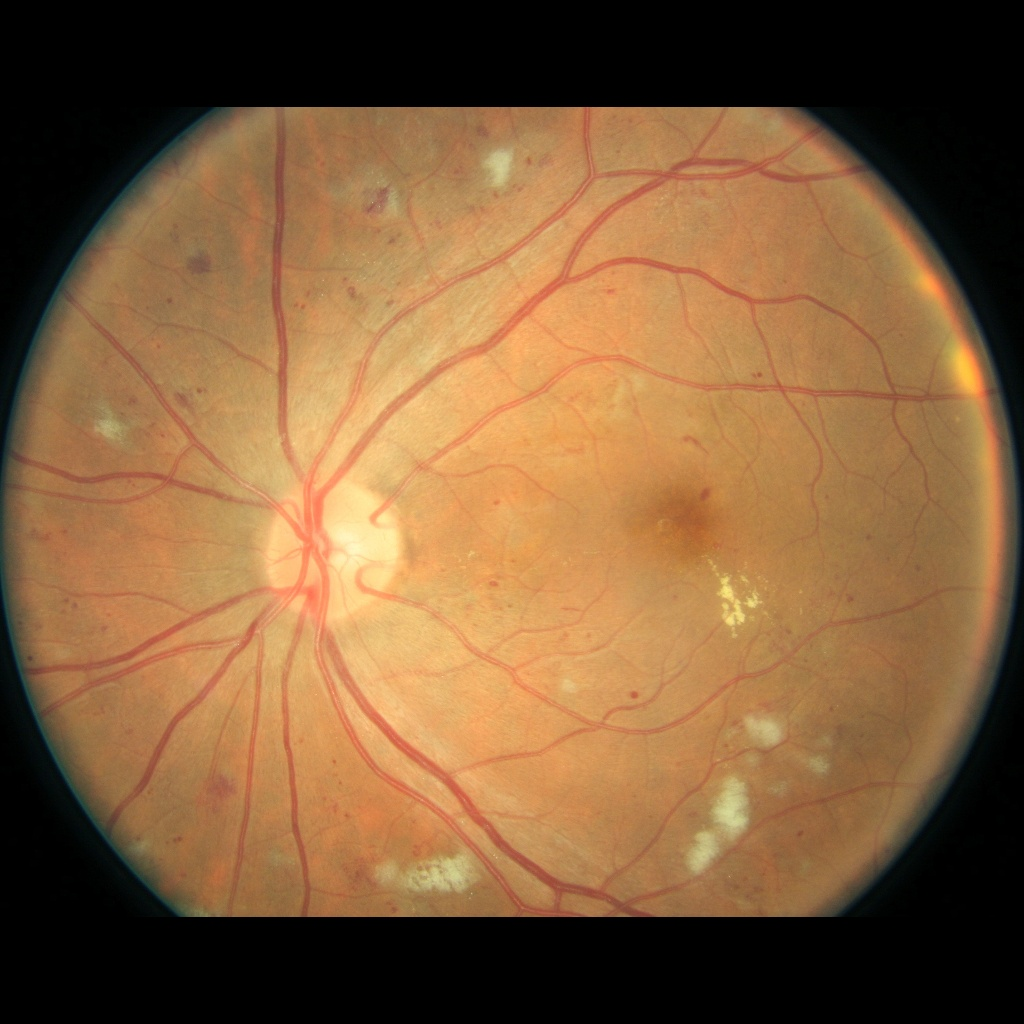
\includegraphics[width=0.2\textwidth]{pics/classified_samples/687_right_3.jpg} &
	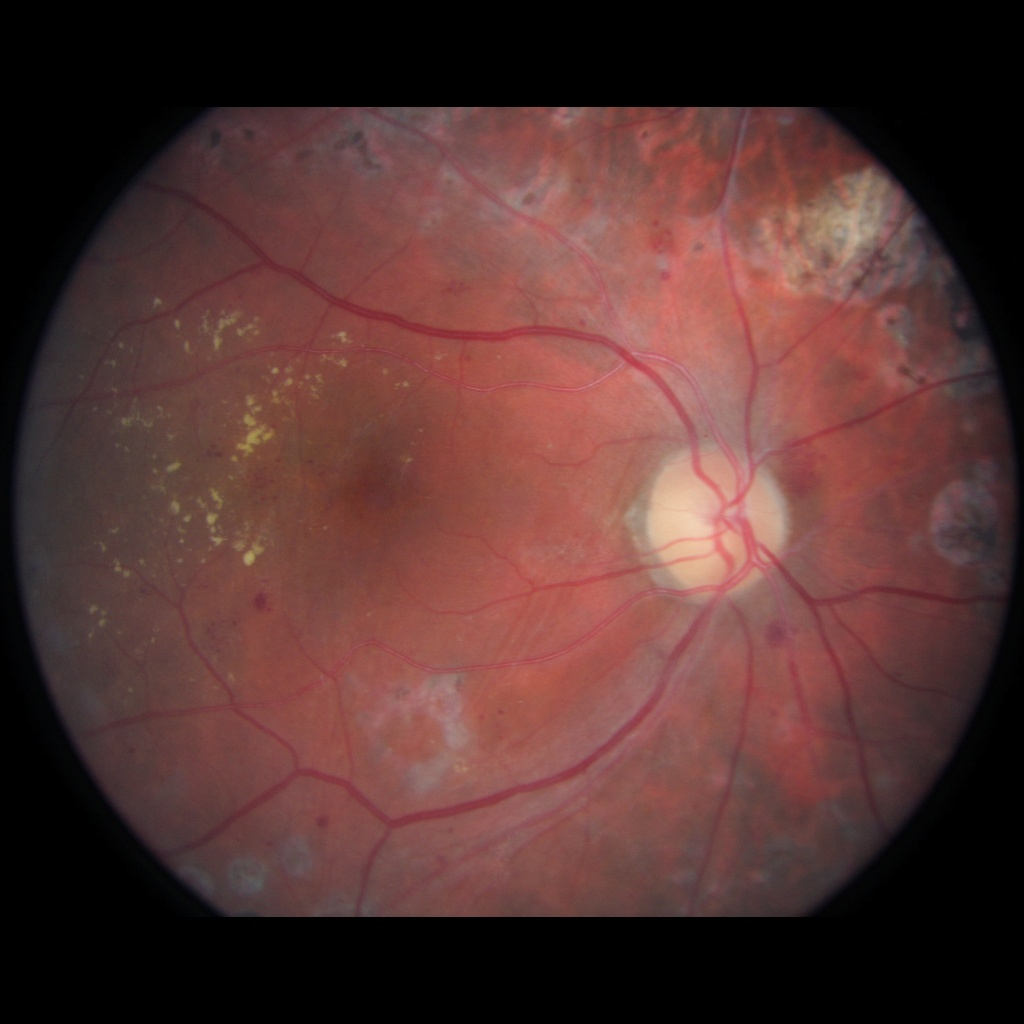
\includegraphics[width=0.2\textwidth]{pics/classified_samples/2496_left_4.jpg} \\\noalign{\vspace{-0.15cm}}
\hline
	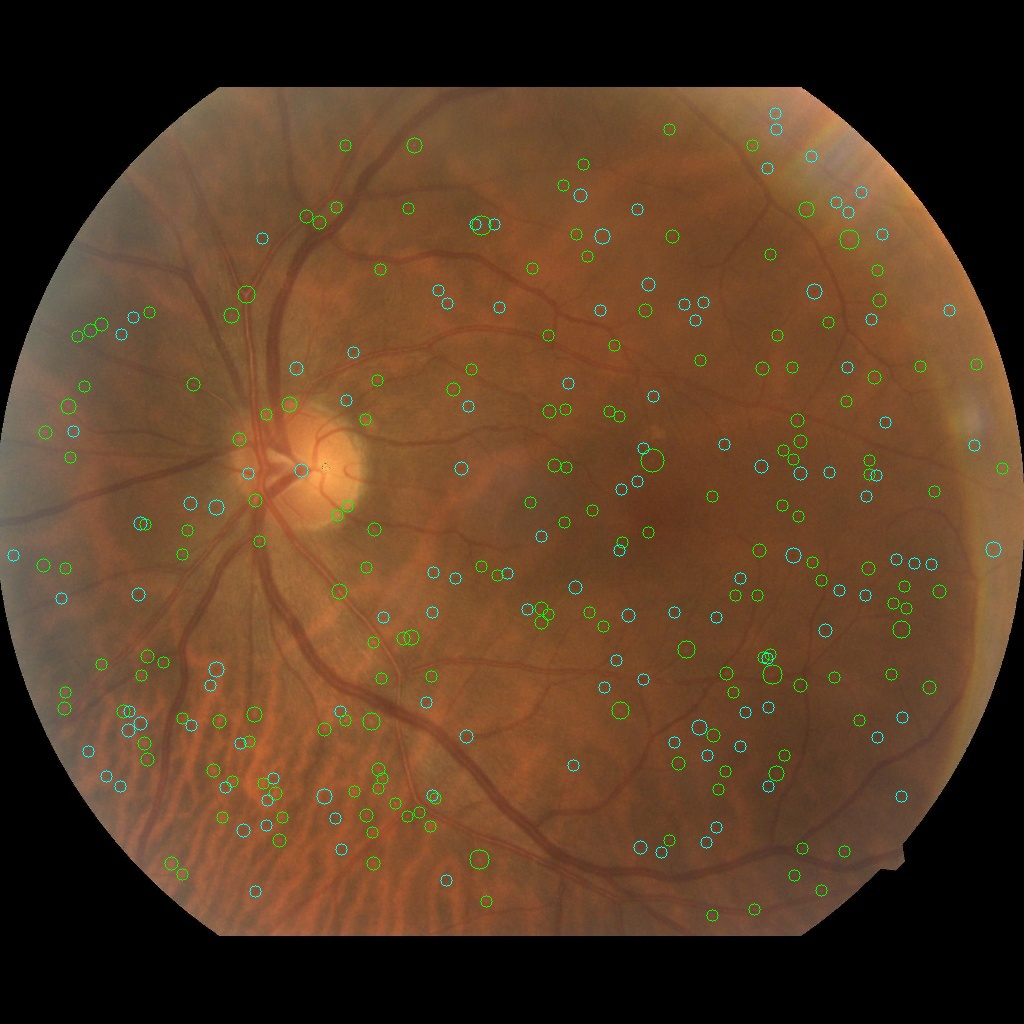
\includegraphics[width=0.2\textwidth]{pics/classified_samples/197_left_0_blobs.jpg} &
	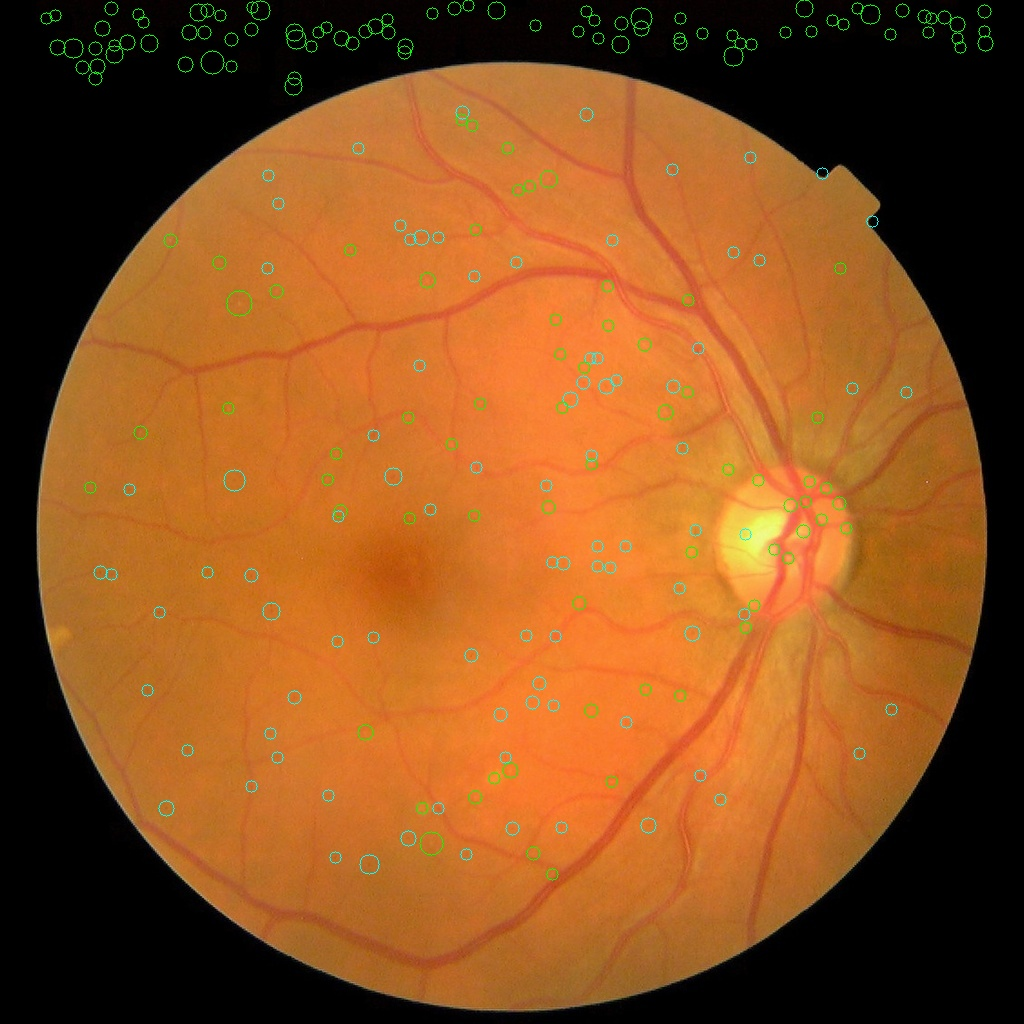
\includegraphics[width=0.2\textwidth]{pics/classified_samples/204_right_1_blobs.jpg} &
	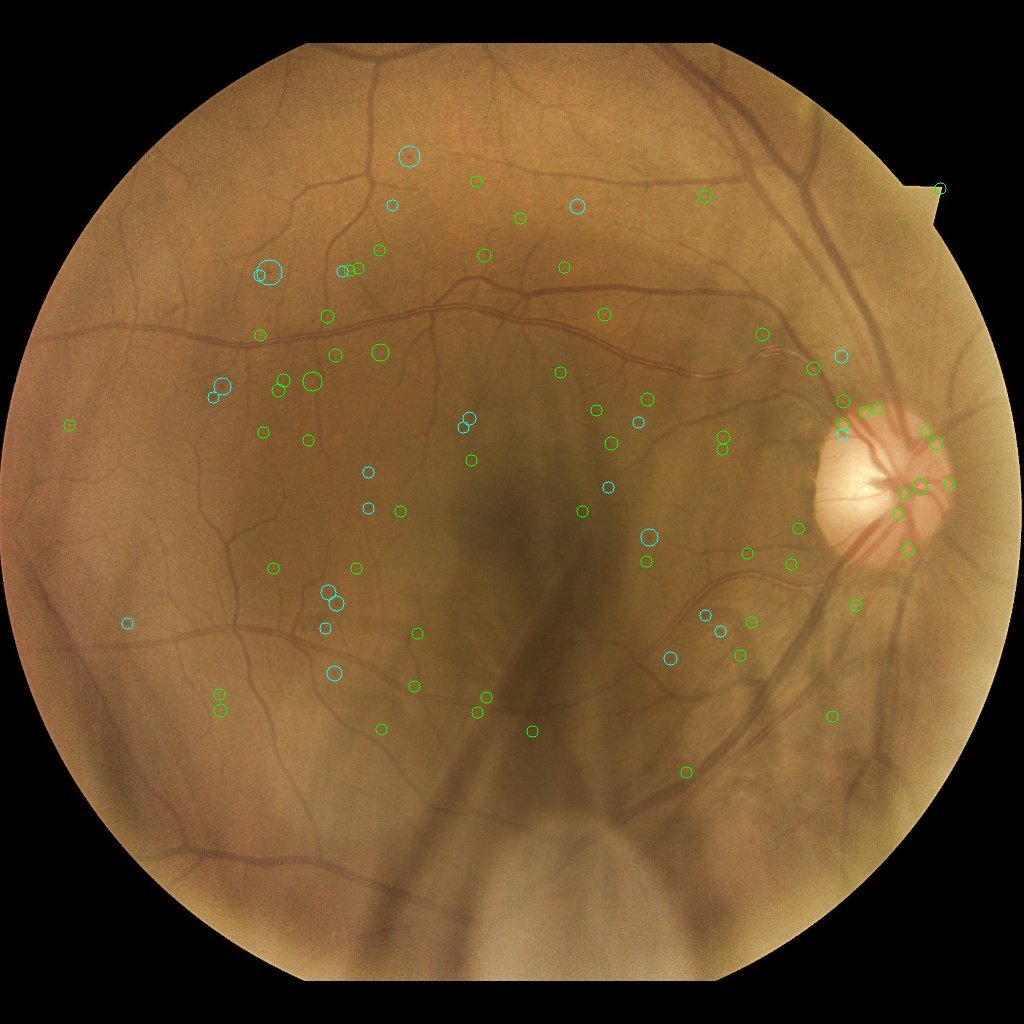
\includegraphics[width=0.2\textwidth]{pics/classified_samples/82_right_2_blobs.jpg} &
	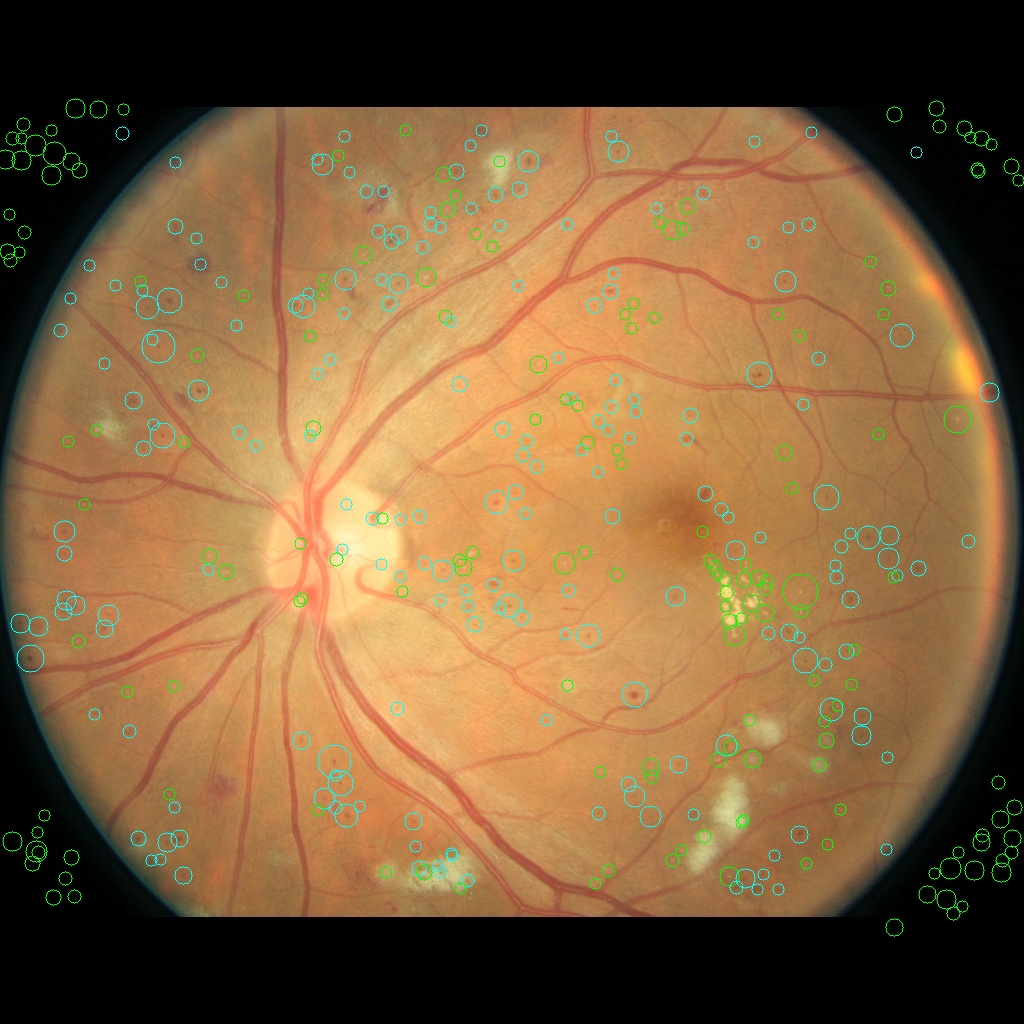
\includegraphics[width=0.2\textwidth]{pics/classified_samples/687_right_3_blobs.jpg} &
	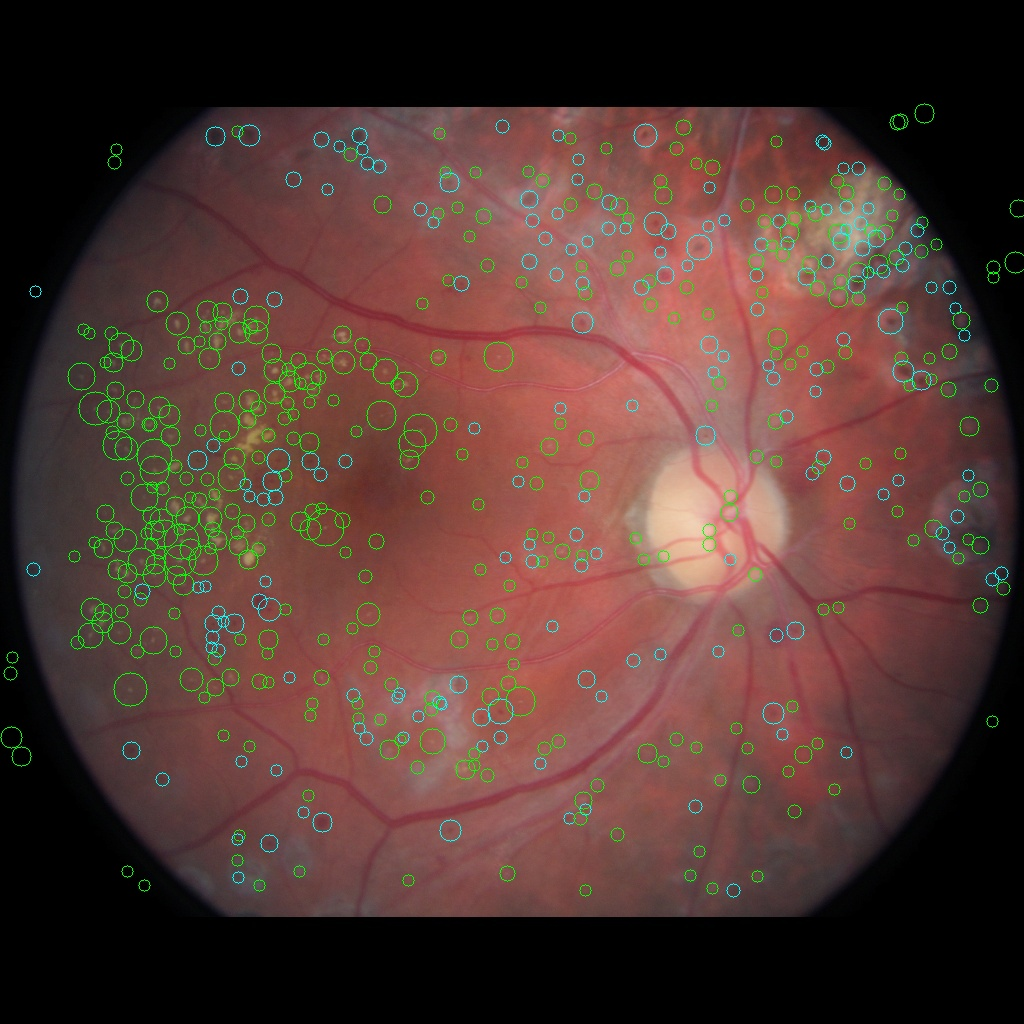
\includegraphics[width=0.2\textwidth]{pics/classified_samples/2496_left_4_blobs.jpg} \\

\end{tabular}
}

\only<2>{
	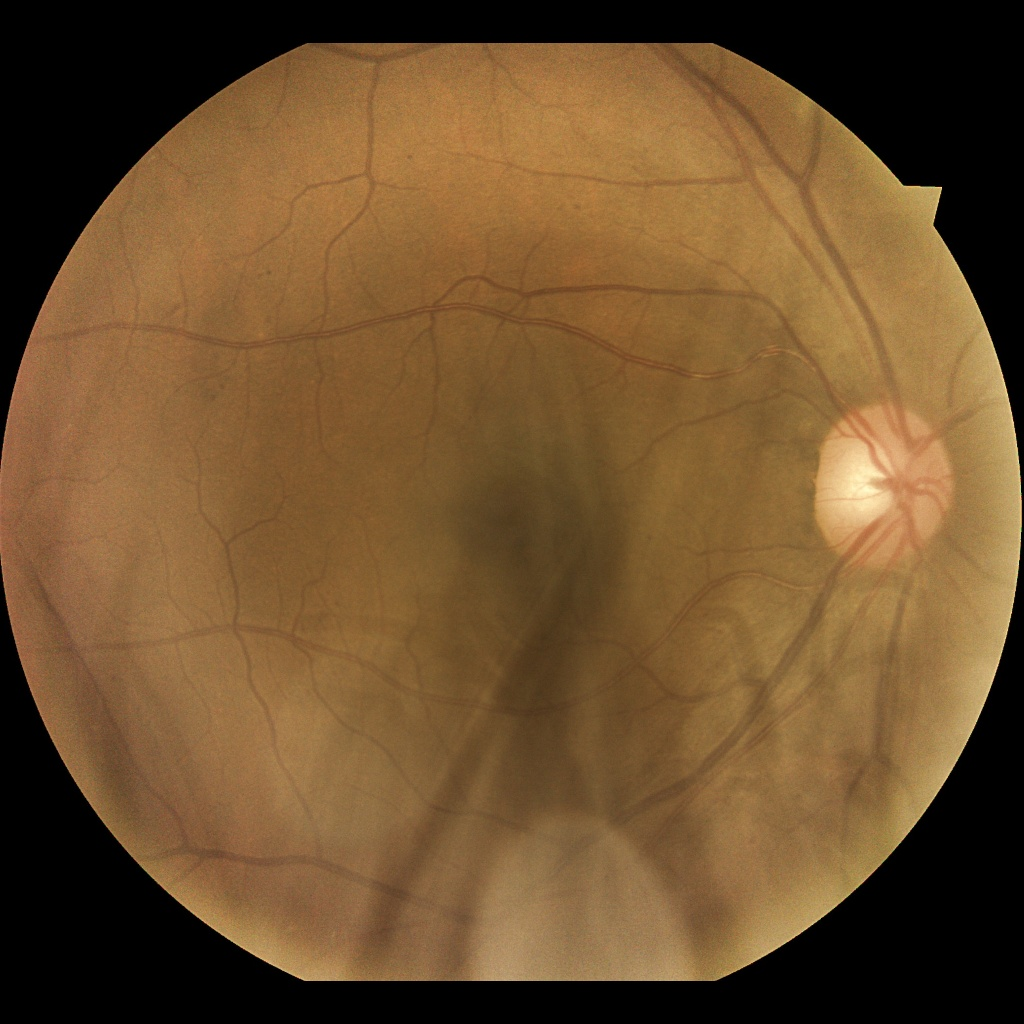
\includegraphics[width=0.65\textwidth]{pics/classified_samples/82_right_2.jpg}
}

\only<3>{
	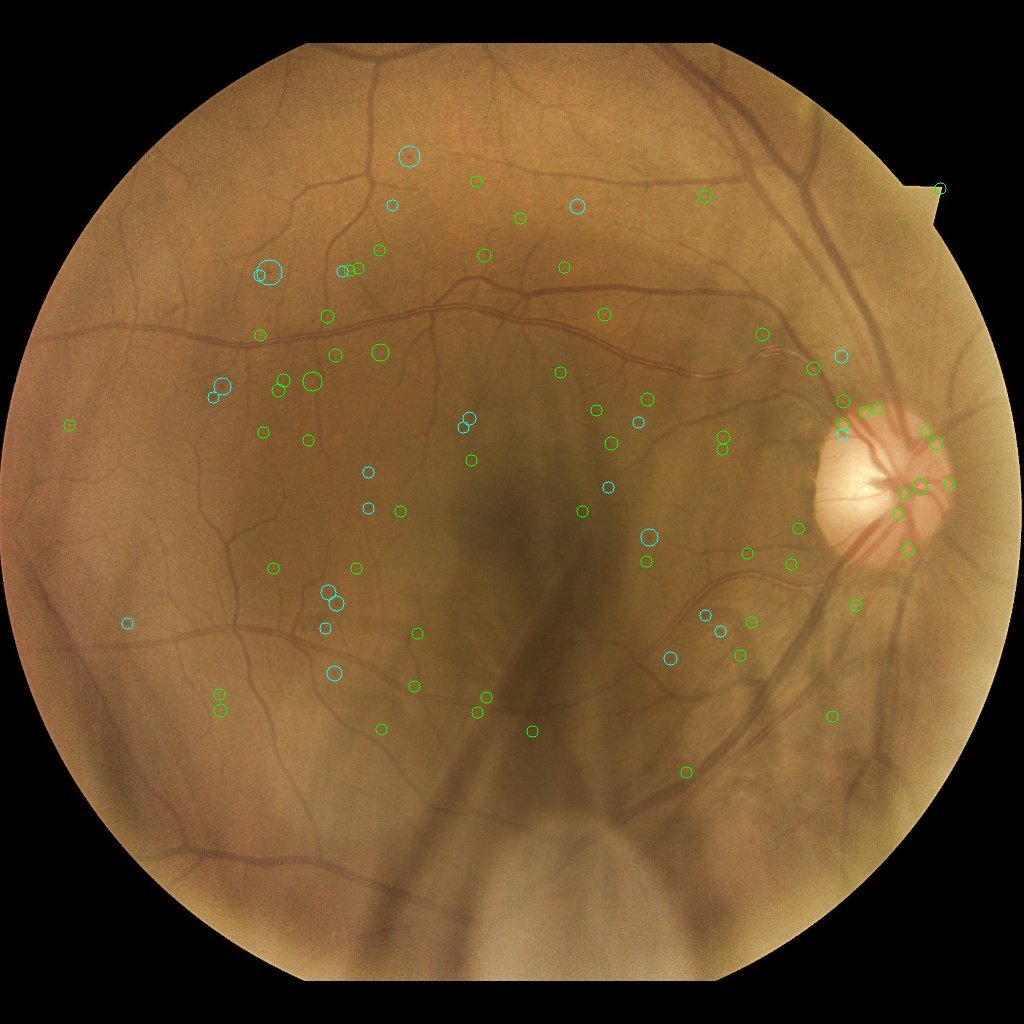
\includegraphics[width=0.65\textwidth]{pics/classified_samples/82_right_2_blobs.jpg}
}
	
\end{frame}

\begin{frame}\frametitle{How blobs looks}

\begin{center}
\begin{tabular}{| b{0.15\linewidth} |@{}c@{}|@{}c@{}|@{}c@{}|@{}c@{}|@{}c@{}|}
\hline
strength & $\sigma = 1.7$ & $\sigma = 3.4$ & $\sigma =  5.1$ & $\sigma = 6.8$ & $\sigma = 8.0$ \\

\hline
$[300,450)$ & 
	\includepatches{patches_300_450_1_2_raw.pdf} & 
	\includepatches{patches_300_450_3_4_raw.pdf} & 
	\includepatches{patches_300_450_5_6_raw.pdf} & 
	\includepatches{patches_300_450_6_7_raw.pdf} & 
	\includepatches{patches_300_450_7_9_raw.pdf} \\

\hline
$[450, 600)$ & 
	\includepatches{patches_450_600_1_2_raw.pdf} & 
	\includepatches{patches_450_600_3_4_raw.pdf} & 
	\includepatches{patches_450_600_5_6_raw.pdf} & 
	\includepatches{patches_450_600_6_7_raw.pdf} & 
	\includepatches{patches_450_600_7_9_raw.pdf} \\
	
\hline
$[600, 750)$ & 
	\includepatches{patches_600_750_1_2_raw.pdf} & 
	\includepatches{patches_600_750_3_4_raw.pdf} & 
	\includepatches{patches_600_750_5_6_raw.pdf} & 
	\includepatches{patches_600_750_6_7_raw.pdf} & 
	\includepatches{patches_600_750_7_9_raw.pdf} \\

\hline
$[750, \infty)$ & 
	\includepatches{patches_750_5000_1_2_raw.pdf} & 
	\includepatches{patches_750_5000_3_4_raw.pdf} & 
	\includepatches{patches_750_5000_5_6_raw.pdf} & 
	\includepatches{patches_750_5000_6_7_raw.pdf} & 
	\\

\hline
\end{tabular}
\end{center}
\end{frame}


\begin{frame}\frametitle{How blobs looks}

\begin{center}
\begin{tabular}{| b{0.15\linewidth} |@{}c@{}|@{}c@{}|@{}c@{}|@{}c@{}|@{}c@{}|}
\hline
strength & $\sigma = 1.7$ & $\sigma = 3.4$ & $\sigma =  5.1$ & $\sigma = 6.8$ & $\sigma = 8.0$ \\

\hline
$[300,450)$ & 
	\includepatches{patches_300_450_1_2_scaled.pdf} & 
	\includepatches{patches_300_450_3_4_scaled.pdf} & 
	\includepatches{patches_300_450_5_6_scaled.pdf} & 
	\includepatches{patches_300_450_6_7_scaled.pdf} & 
	\includepatches{patches_300_450_7_9_scaled.pdf} \\

\hline
$[450, 600)$ & 
	\includepatches{patches_450_600_1_2_scaled.pdf} & 
	\includepatches{patches_450_600_3_4_scaled.pdf} & 
	\includepatches{patches_450_600_5_6_scaled.pdf} & 
	\includepatches{patches_450_600_6_7_scaled.pdf} & 
	\includepatches{patches_450_600_7_9_scaled.pdf} \\
	
\hline
$[600, 750)$ & 
	\includepatches{patches_600_750_1_2_scaled.pdf} & 
	\includepatches{patches_600_750_3_4_scaled.pdf} & 
	\includepatches{patches_600_750_5_6_scaled.pdf} & 
	\includepatches{patches_600_750_6_7_scaled.pdf} & 
	\includepatches{patches_600_750_7_9_scaled.pdf} \\

\hline
$[750, \infty)$ & 
	\includepatches{patches_750_5000_1_2_scaled.pdf} & 
	\includepatches{patches_750_5000_3_4_scaled.pdf} & 
	\includepatches{patches_750_5000_5_6_scaled.pdf} & 
	\includepatches{patches_750_5000_6_7_scaled.pdf} & 
	\\

\hline
\end{tabular}
\end{center}
\end{frame}

\subsection{Bag of visual words}
\begin{frame}\frametitle{BoVW preparation}
\begin{itemize}
\item Extract local descriptors from blob patch: HOG, LBP
\item K-means segmentation for quantization
\item Use histograms of visual words as feature vectors
\end{itemize}
\end{frame}

\begin{frame}\frametitle{BoVW preparation}
\par Unfortunately I got stuck on this point two weeks before challenge deadline. :-(
\begin{center}
\begin{figure}
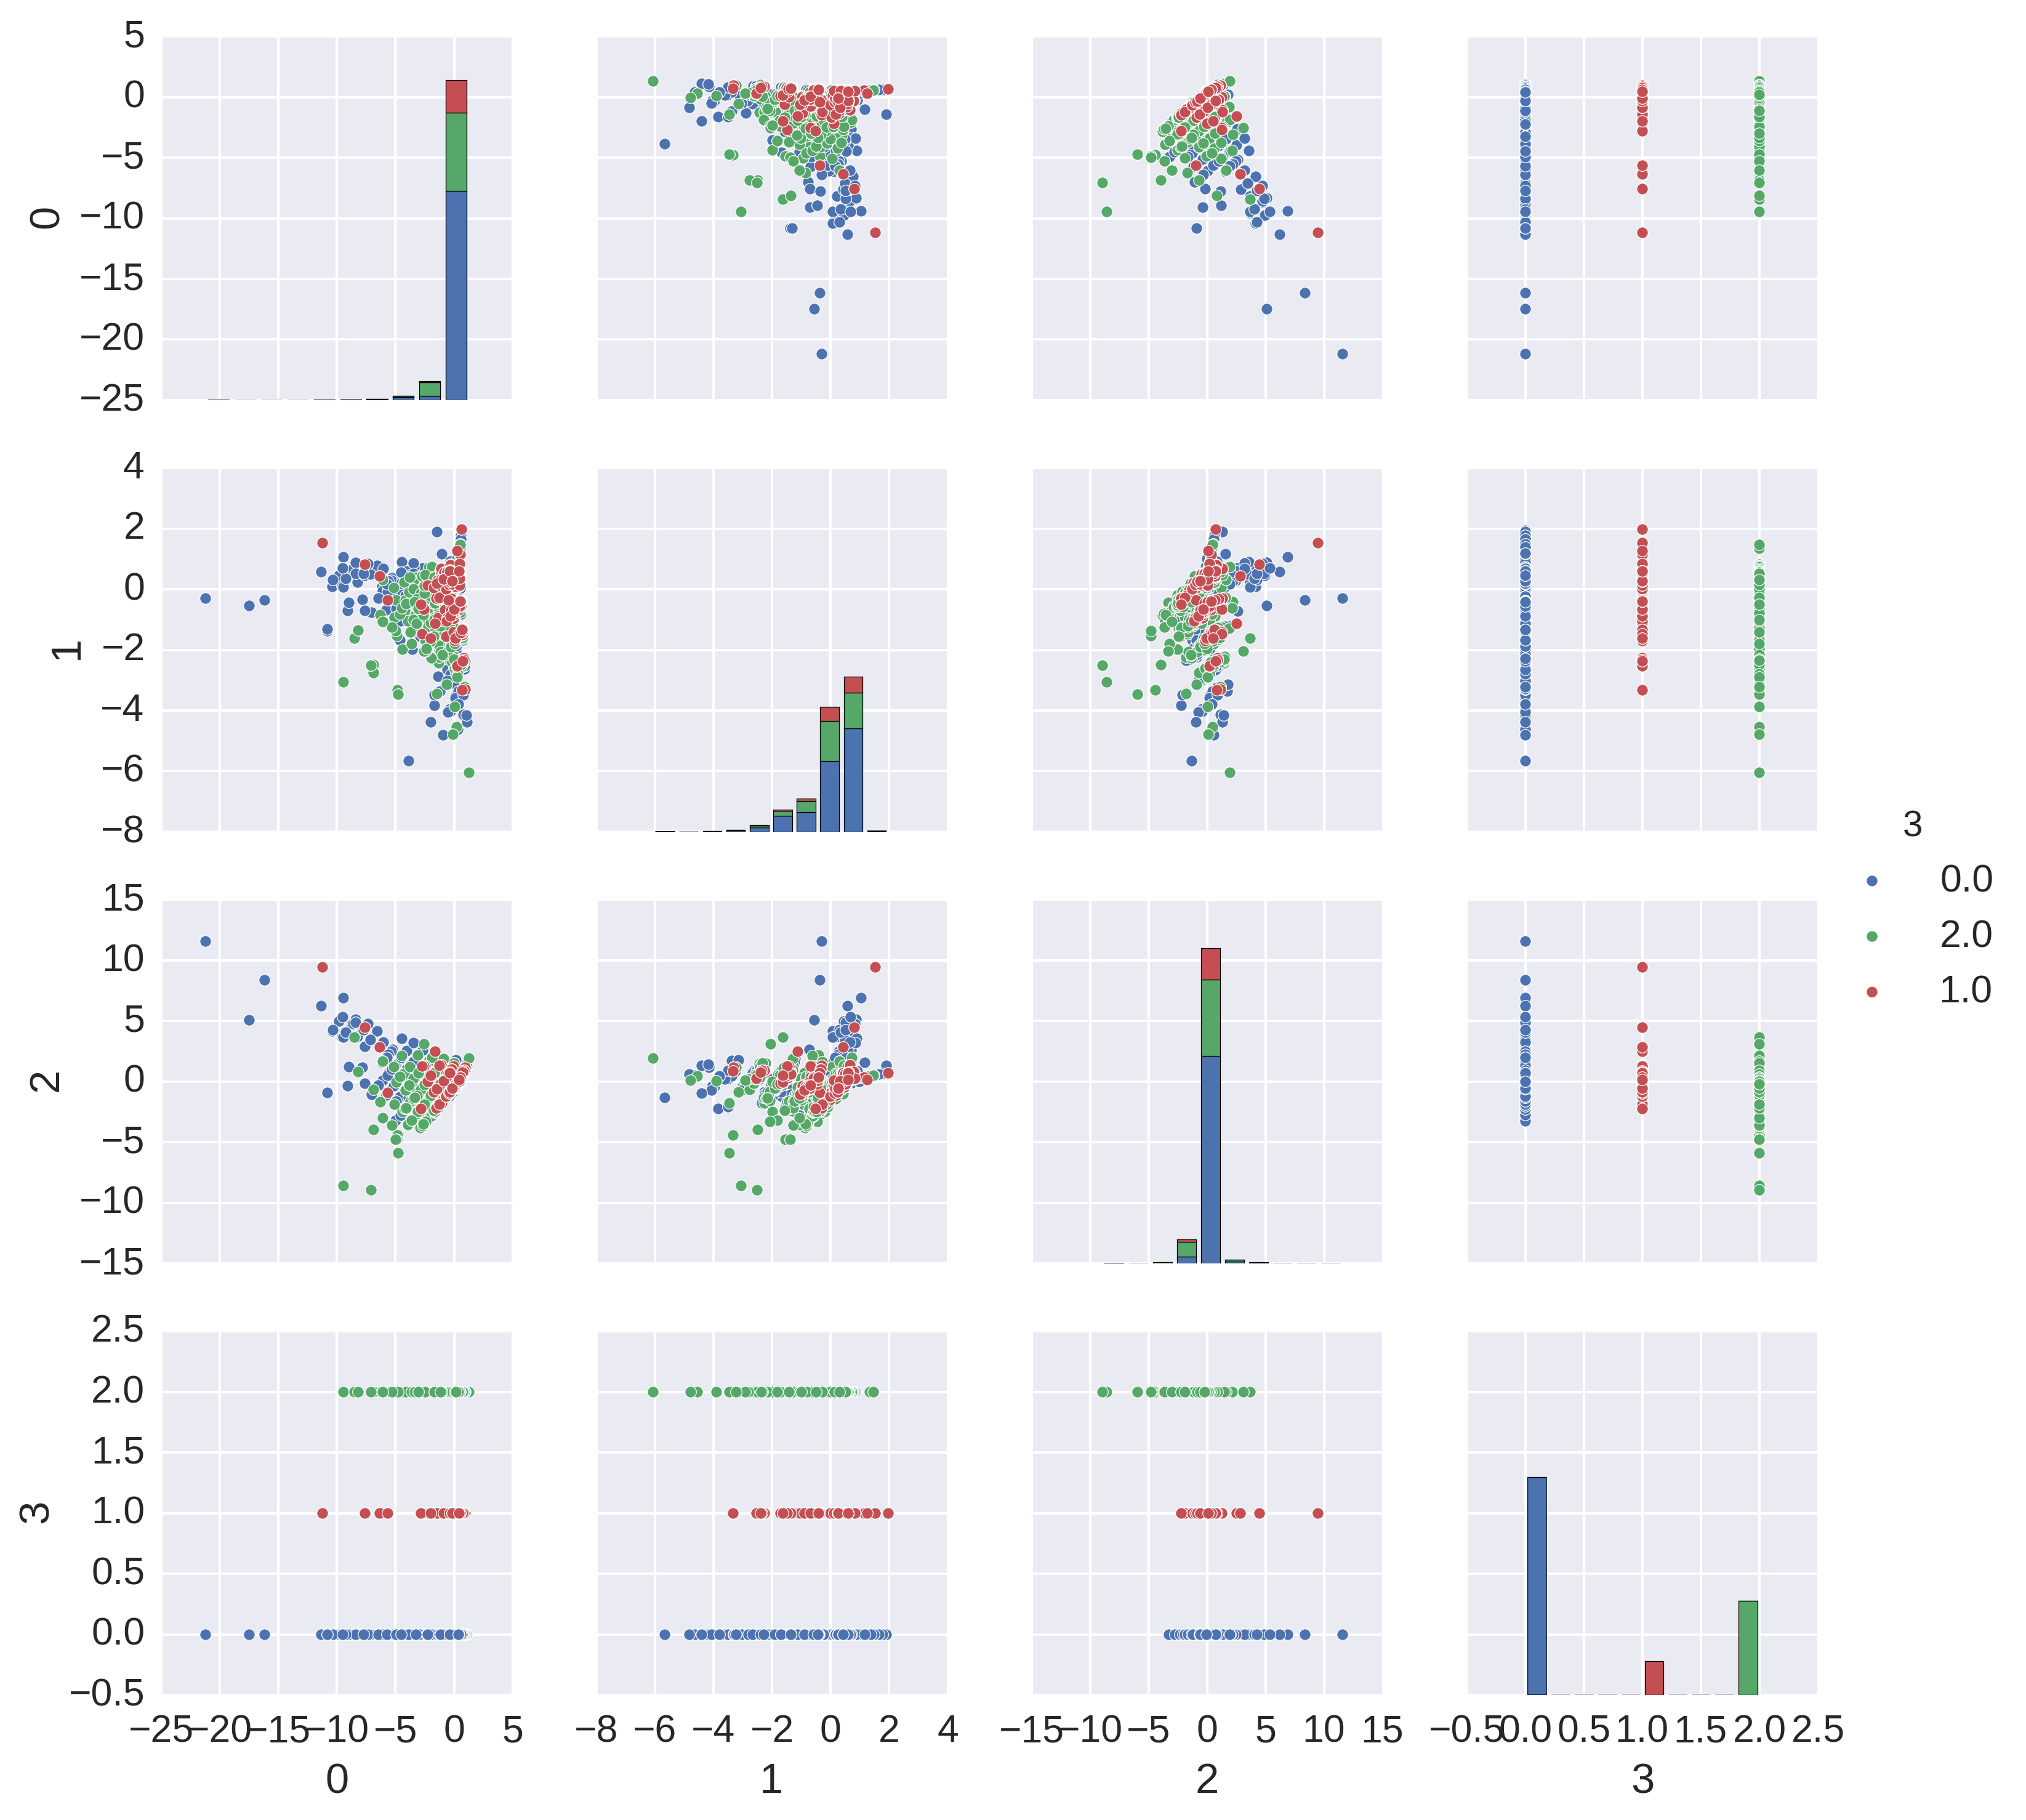
\includegraphics[width=0.5\textwidth]{pics/bow_pca_results.png}
\caption{Typical picture of BoW features  after applying PCA.}
\end{figure}
\end{center}
\end{frame}
% % % %
% % % % Conclusions
% % % %
\section{Conclusions}
\begin{frame}\frametitle{Conclusions}
\begin{itemize}

% What the Fuck?
\item Teamwork
\begin{itemize}
\item Find good tools for effective collaboration
\item Divide and conquer
\item Learn together
\item Maintain model diversity
\end{itemize}

\item Competition
\begin{itemize}
\item Setup a reliable experiment-evaluate loop
\item Be careful when keeping track of experiments
\item Plan ahead when experiments are long (24+ hours in out case)
\item Understand evaluation metric
\item Try different things
\end{itemize}

\end{itemize}
\end{frame}
% % % %
% % % % Winner's approaches
% % % %
% \section{Winner's approaches} 
% %\subsection{\nth{1} place}
% \begin{frame}\frametitle{\nth{1} place}
% \end{frame}
% %\subsection{\nth{2} place}
% \begin{frame}\frametitle{\nth{2} place}
% \end{frame}
% %\subsection{\nth{3} place}
% \begin{frame}\frametitle{\nth{3} place}
% \end{frame}


%
%
% Back up
% There are examples below to use in slides
%

%\section{Back Up}
%
%\begin{frame}\frametitle{Tables}
%\begin{tabular}{|c|c|c|}
%\hline
%\textbf{Date} & \textbf{Instructor} & \textbf{Title} \\
%\hline
%WS 04/05 & Sascha Frank & First steps with  \LaTeX  \\
%\hline
%SS 05 & Sascha Frank & \LaTeX \ Course serial \\
%\hline
%\end{tabular}
%\end{frame}
%
%%\subsection{blocs}
%\begin{frame}\frametitle{blocs}
%
%\begin{block}{title of the bloc1}
%bloc text
%\end{block}
%
%\begin{exampleblock}{title of the bloc2}
%bloc text
%\end{exampleblock}
%
%
%\begin{alertblock}{title of the bloc3}
%bloc text
%\end{alertblock}
%
%\end{frame}
%
%%\subsection{split screen}
%
%\begin{frame}\frametitle{splitting screen}
%\begin{columns}
%\begin{column}{5cm}
%\begin{itemize}
%\item Beamer 
%\item Beamer Class 
%\item Beamer Class Latex 
%\end{itemize}
%\end{column}
%\begin{column}{5cm}
%\begin{tabular}{|c|c|}
%\hline
%\textbf{Instructor} & \textbf{Title} \\
%\hline
%Sascha Frank &  \LaTeX \ Course 1 \\
%\hline
%Sascha Frank &  Course serial  \\
%\hline
%\end{tabular}
%\end{column}
%\end{columns}
%\end{frame}
%
%%\subsection{Pictures} 
%\begin{frame}\frametitle{pictures in latex beamer class}
%\begin{figure}
%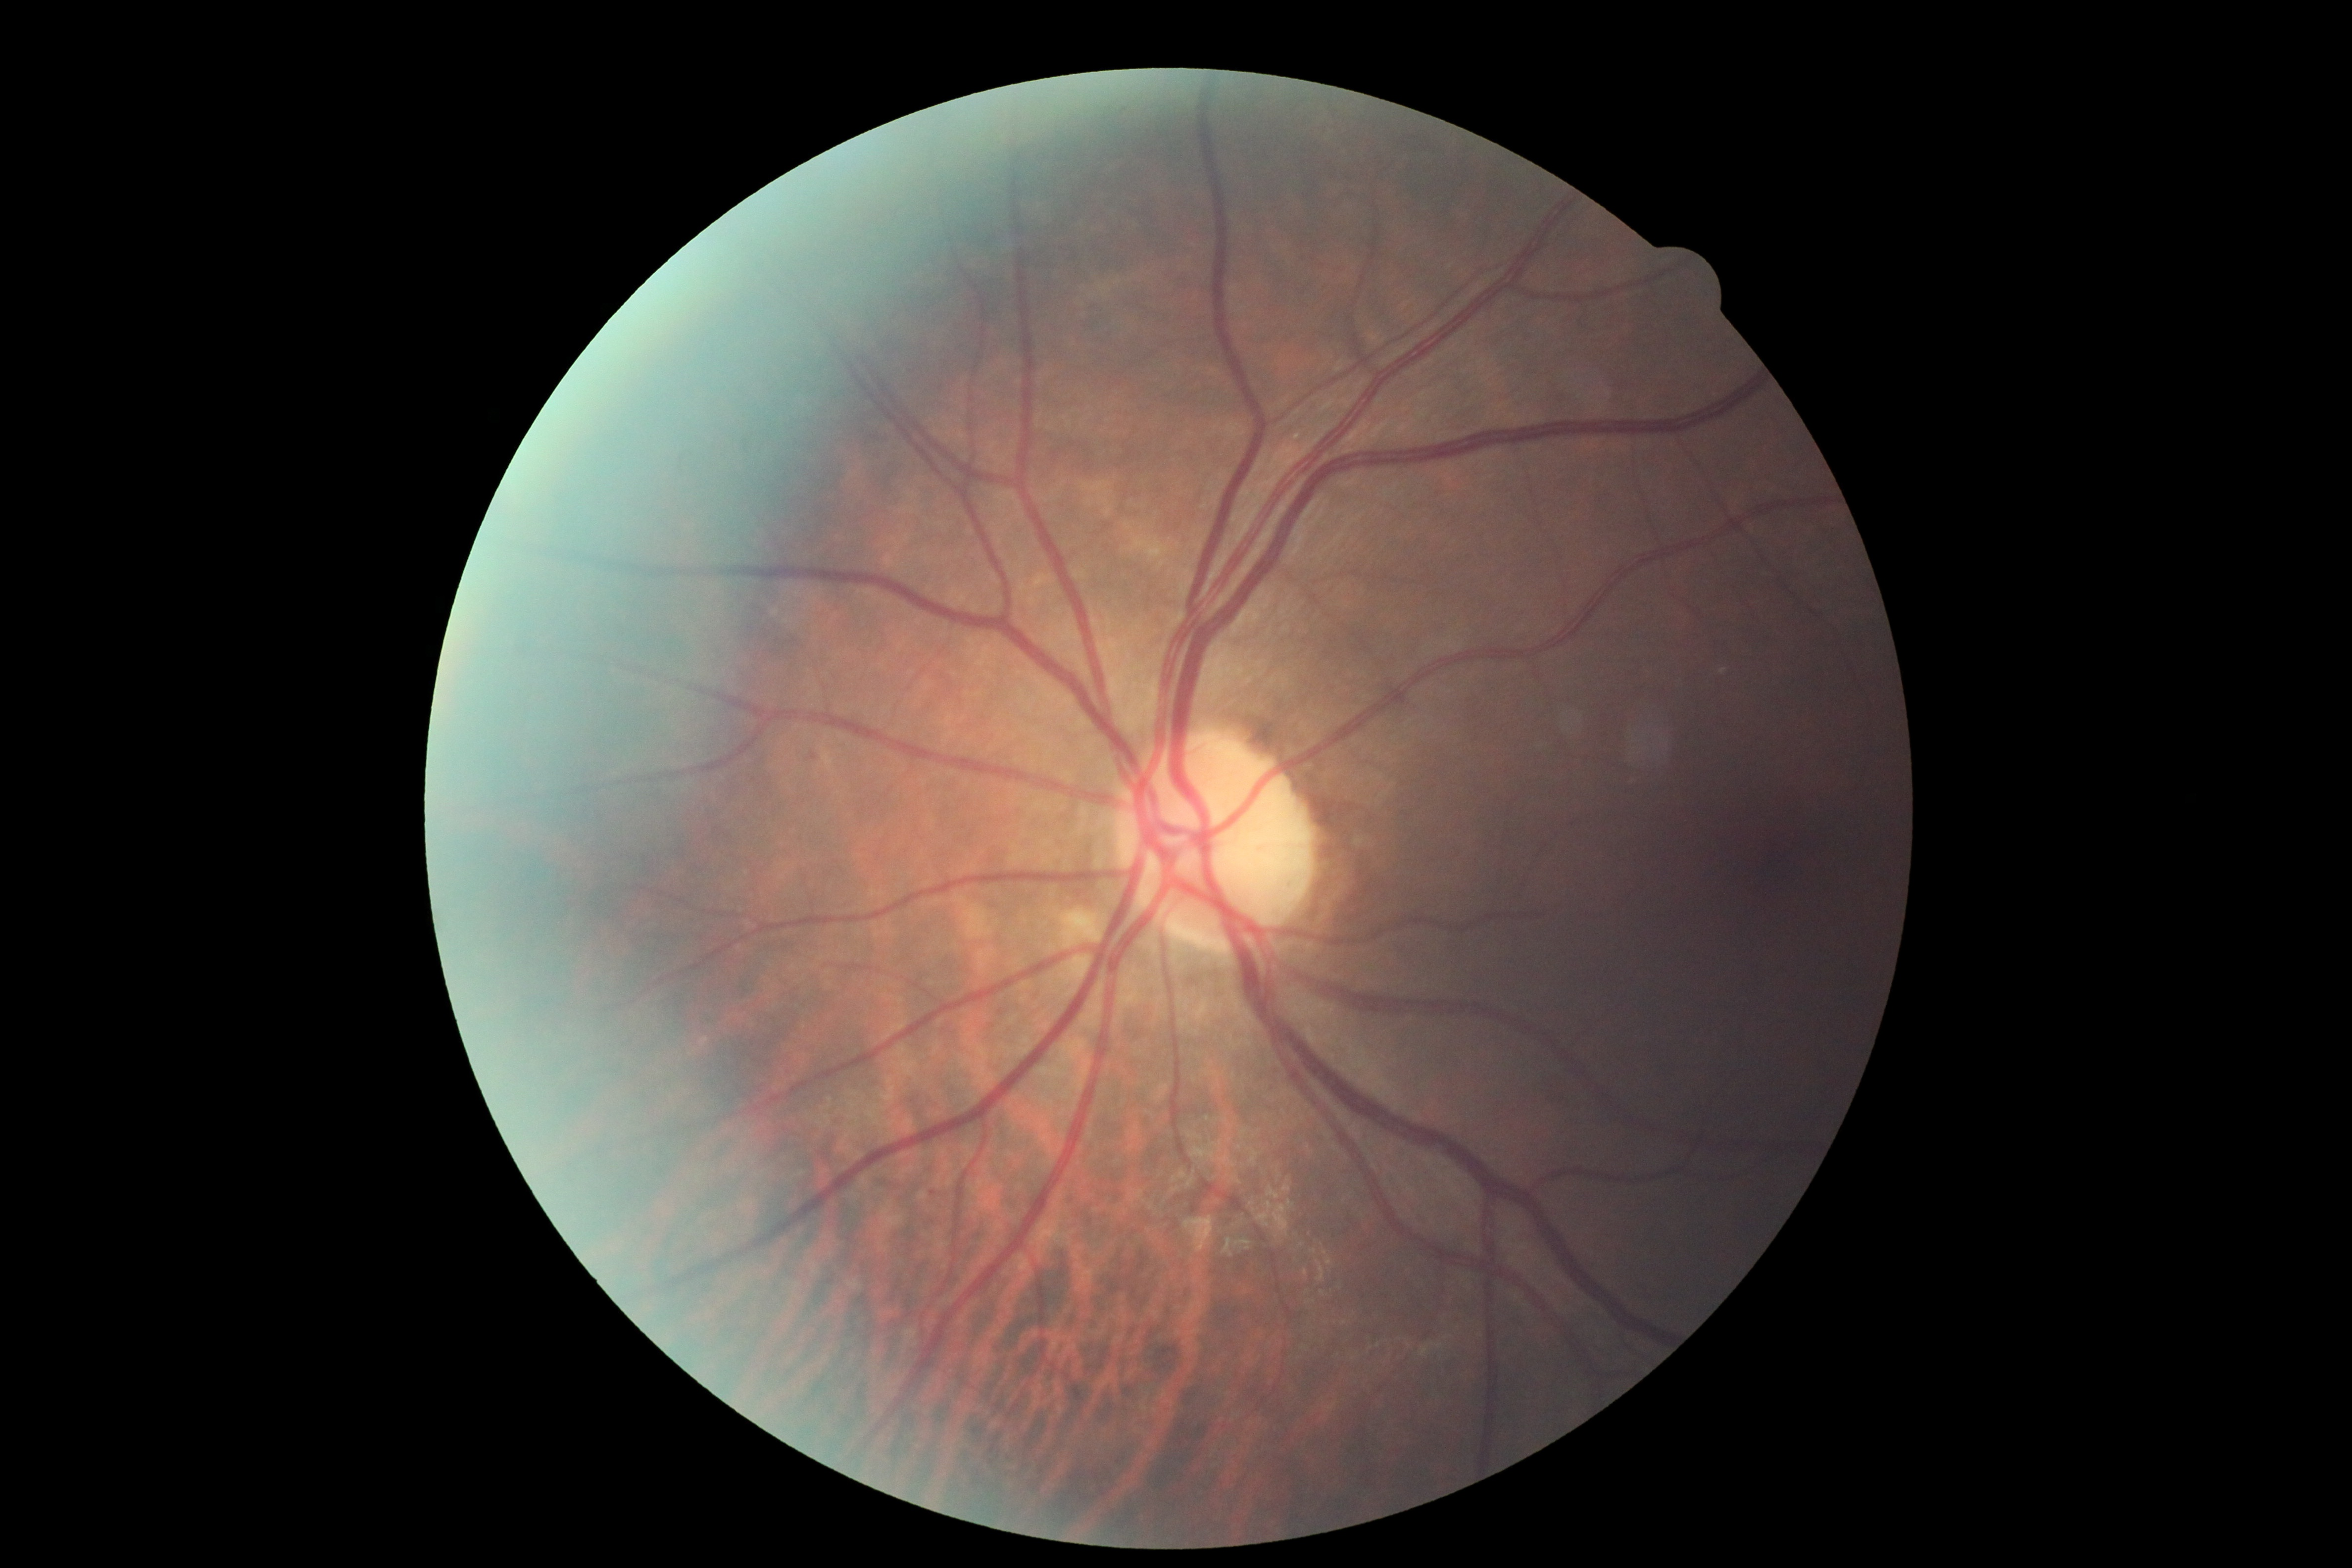
\includegraphics[scale=0.5]{pics/10_left.jpeg} 
%\caption{show an example picture}
%\end{figure}
%\end{frame}
%
%%\subsection{joining picture and lists} 
%
%\begin{frame}
%\frametitle{pictures and lists in beamer class}
%\begin{columns}
%\begin{column}{5cm}
%\begin{itemize}
%\item<1-> subject 1
%\item<3-> subject 2
%\item<5-> subject 3
%\end{itemize}
%\vspace{3cm} 
%\end{column}
%\begin{column}{5cm}
%\begin{overprint}
%\includegraphics<2>[width=2.5cm]{pics/10_left.jpeg}
%\includegraphics<4>[width=2.5cm]{pics/10_left.jpeg}
%\includegraphics<6>[width=2.5cm]{pics/10_left.jpeg}
%\end{overprint}
%\end{column}
%\end{columns}
%\end{frame}
%
%
%%\subsection{pictures which need more space} 
%\begin{frame}[plain]
%\frametitle{plain, or a way to get more space}
%\begin{figure}
%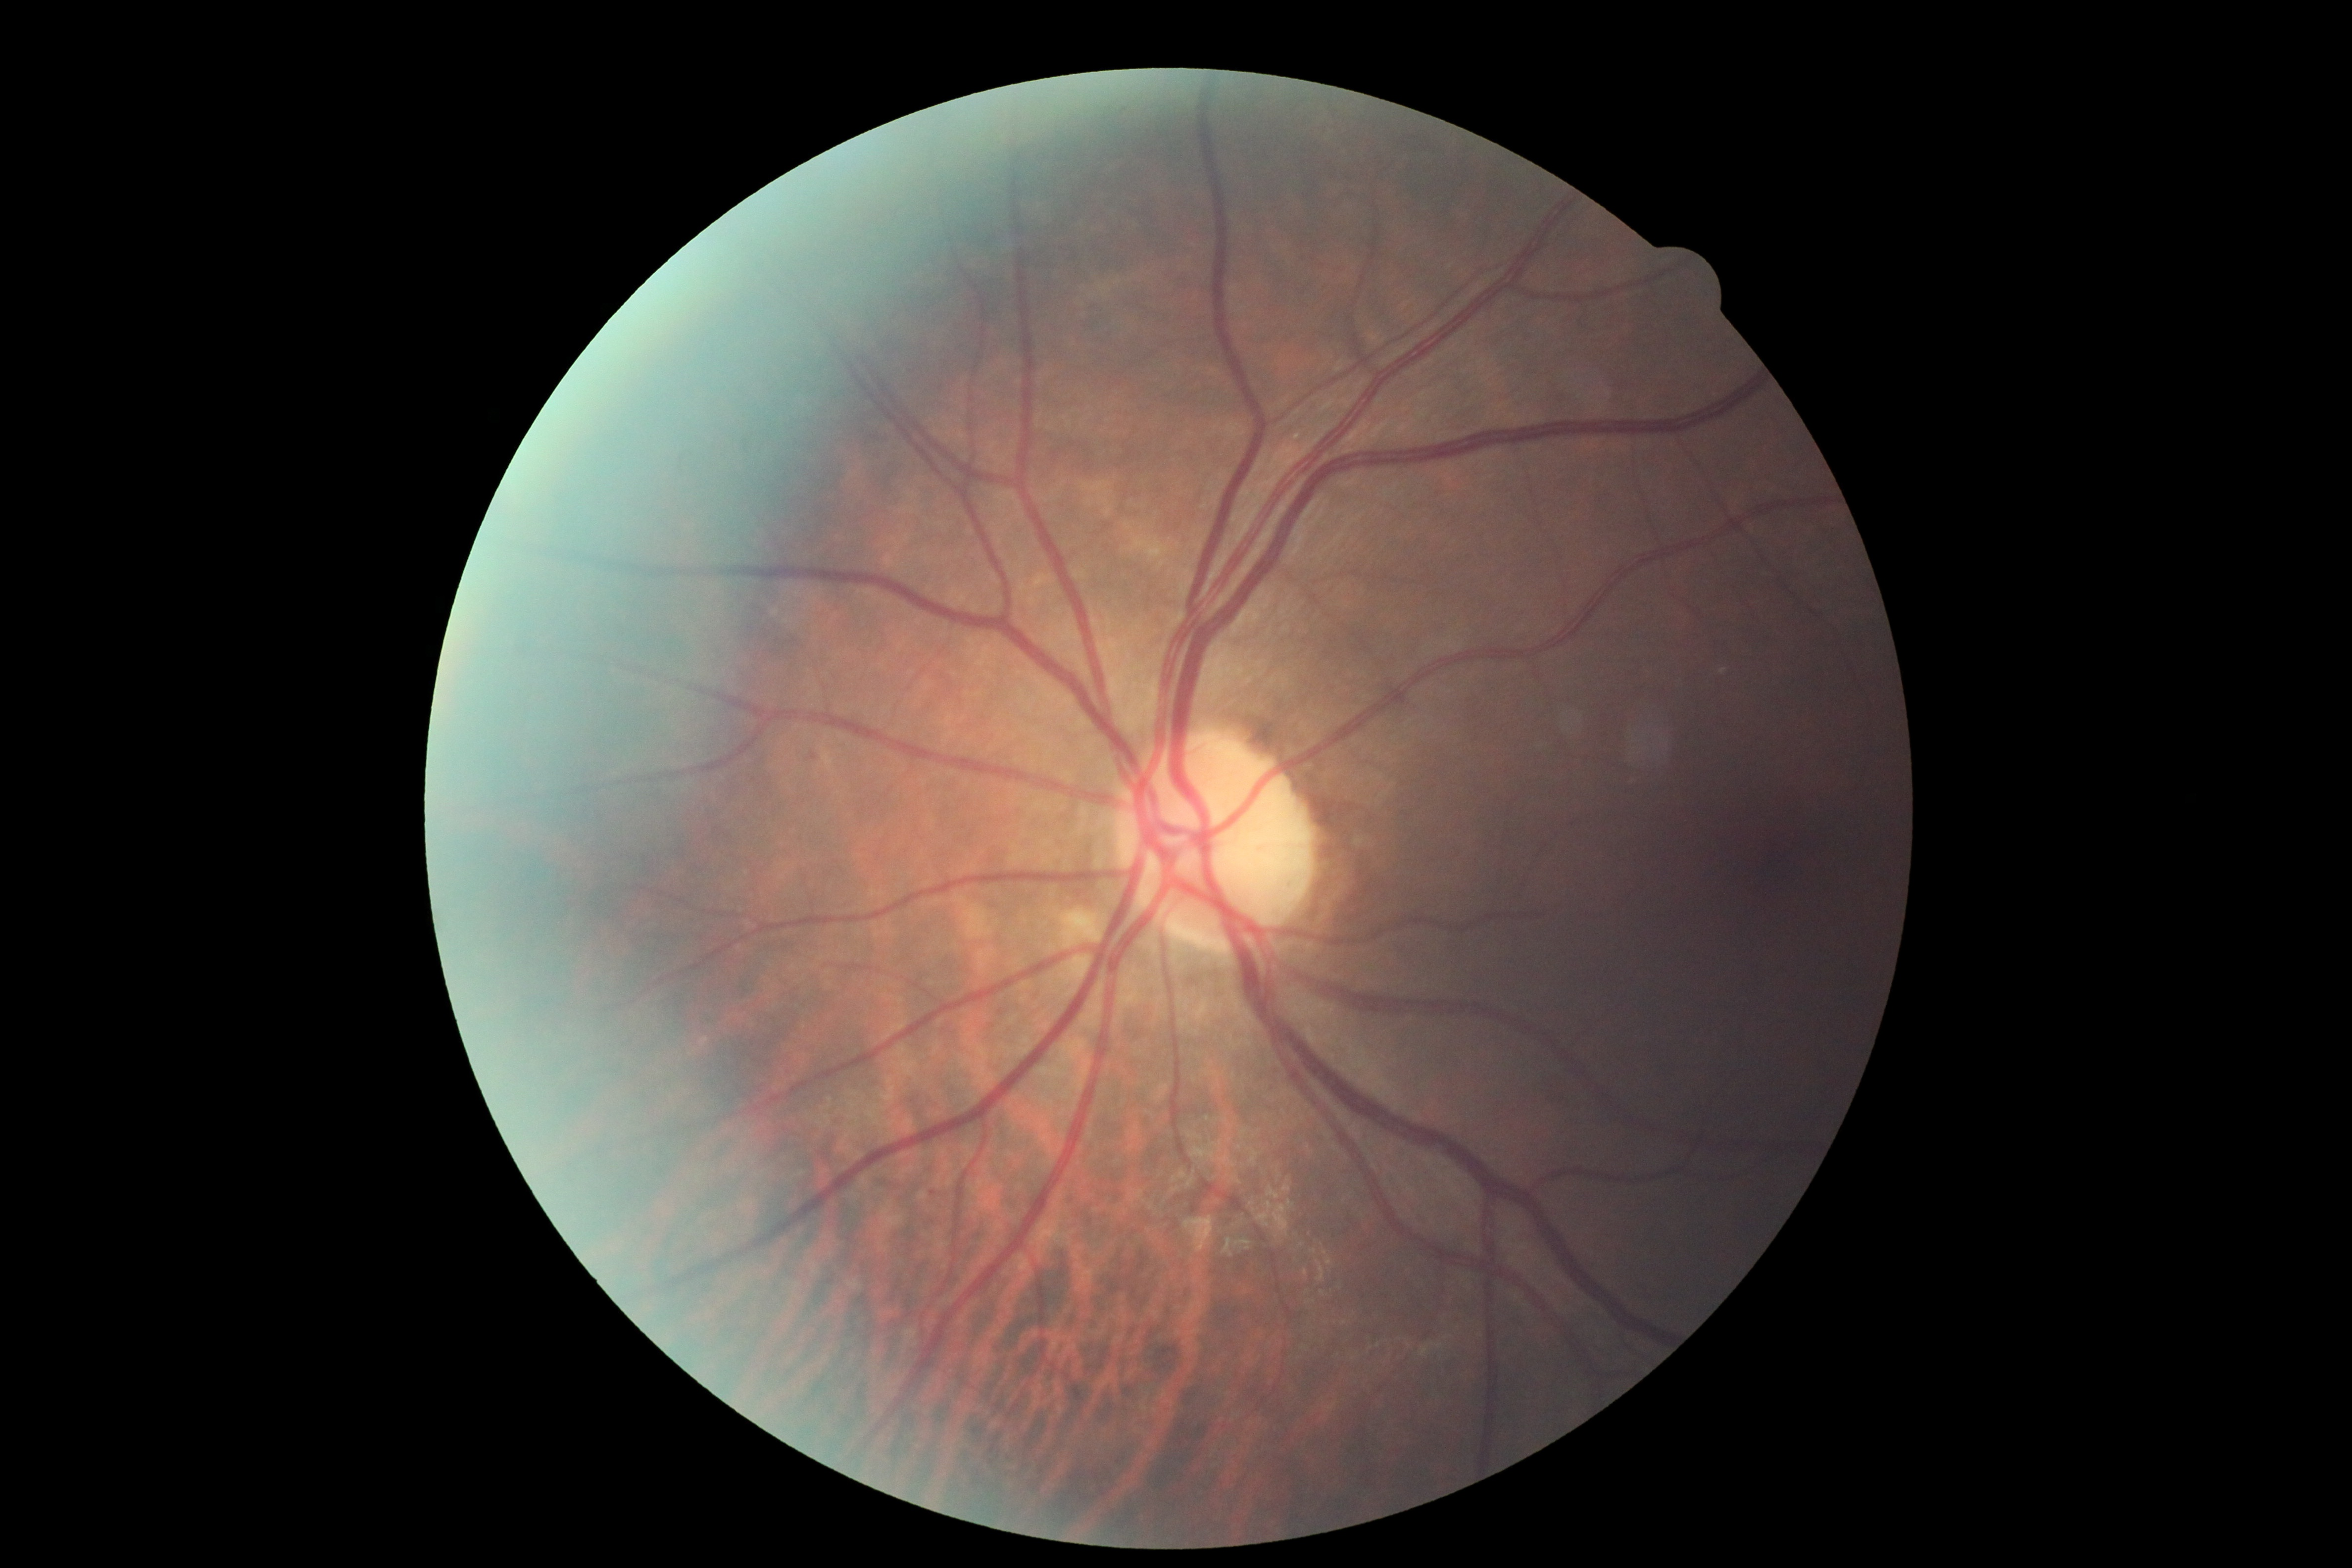
\includegraphics[scale=0.25]{pics/10_left.jpeg} 
%\caption{show an example picture}
%\end{figure}
%\end{frame}
%
%
%
%
%
%

\end{document}